%&preformat-present

\newif\ifpresentation % Условие, проверяющее, что документ --- презентация
\presentationtrue
\documentclass[8pt, xcolor={dvipsnames, table, hyperref}]{beamer}

%%%%%%%%%%%%%%%%%%%%%%%%%%%%%%%%%%%%%%%%%%%%%%%%%%%%%%%%%%%%%%%%%%%%%%%%%%%%%%%%
%%%% Файл упрощённых настроек шаблона, общих для диссертации и автореферата %%%%
%%%%%%%%%%%%%%%%%%%%%%%%%%%%%%%%%%%%%%%%%%%%%%%%%%%%%%%%%%%%%%%%%%%%%%%%%%%%%%%%

%%% Режим черновика %%%
\makeatletter
\@ifundefined{c@draft}{
  \newcounter{draft}
  \setcounter{draft}{0}  % 0 --- чистовик (максимальное соблюдение ГОСТ)
                         % 1 --- черновик (отклонения от ГОСТ, но быстрая
                         %       сборка итоговых PDF)
}{}
\makeatother

%%% Пометки в тексте %%%
\makeatletter
\@ifundefined{c@showmarkup}{
  \newcounter{showmarkup}
  \setcounter{showmarkup}{1}  % 0 --- скрыть пометки
                              % 1 --- показывать пометки
}{}
\makeatother

%%% Использование в pdflatex шрифтов не по-умолчанию %%%
\makeatletter
\@ifundefined{c@usealtfont}{
  \newcounter{usealtfont}
  \setcounter{usealtfont}{1}    % 0 --- шрифты на базе Computer Modern
                                % 1 --- использовать пакет pscyr, при его
                                %       наличии
                                % 2 --- использовать пакет XCharter, при наличии
                                %       подходящей версии
}{}
\makeatother

%%% Использование в xelatex и lualatex семейств шрифтов %%%
\makeatletter
\@ifundefined{c@fontfamily}{
  \newcounter{fontfamily}
  \setcounter{fontfamily}{2}  % 0 --- CMU семейство. Используется как fallback;
                              % 1 --- Шрифты от MS (Times New Roman и компания)
                              % 2 --- Семейство Liberation
}{}
\makeatother

%%% Библиография %%%
\makeatletter
\@ifundefined{c@bibliosel}{
  \newcounter{bibliosel}
  \setcounter{bibliosel}{1}   % 0 --- встроенная реализация с загрузкой файла
                              %       через движок bibtex8;
                              % 1 --- реализация пакетом biblatex через движок
                              %       biber
}{}
\makeatother

%%% Вывод типов ссылок в библиографии %%%
\makeatletter
\@ifundefined{c@mediadisplay}{
  \newcounter{mediadisplay}
  \setcounter{mediadisplay}{1}   % 0 --- не делать ничего; надписи [Текст] и
                                 %       [Эл. ресурс] будут выводиться только в ссылках с
                                 %       заполненным полем `media`;
                                 % 1 --- автоматически добавлять надпись [Текст] к ссылкам с
                                 %       незаполненным полем `media`; таким образом, у всех
                                 %       источников будет указан тип, что соответствует
                                 %       требованиям ГОСТ
                                 % 2 --- автоматически удалять надписи [Текст], [Эл. Ресурс] и др.;
                                 %       не соответствует ГОСТ
                                 % 3 --- автоматически удалять надпись [Текст];
                                 %       не соответствует ГОСТ
                                 % 4 --- автоматически удалять надпись [Эл. Ресурс];
                                 %       не соответствует ГОСТ
}{}
\makeatother

%%% Предкомпиляция tikz рисунков для ускорения работы %%%
\makeatletter
\@ifundefined{c@imgprecompile}{
  \newcounter{imgprecompile}
  \setcounter{imgprecompile}{0}   % 0 --- без предкомпиляции;
                                  % 1 --- пользоваться предварительно
                                  %       скомпилированными pdf вместо генерации
                                  %       заново из tikz
}{}
\makeatother
               % Общие настройки шаблона
%%% Проверка используемого TeX-движка %%%
\newif\ifxetexorluatex   % определяем новый условный оператор (http://tex.stackexchange.com/a/47579)
\ifxetex
    \xetexorluatextrue
\else
    \ifluatex
        \xetexorluatextrue
    \else
        \xetexorluatexfalse
    \fi
\fi

\newif\ifsynopsis           % Условие, проверяющее, что документ --- автореферат

\usepackage{etoolbox}[2015/08/02]   % Для продвинутой проверки разных условий
\providebool{presentation}

\usepackage{comment}    % Позволяет убирать блоки текста (добавляет
                        % окружение comment и команду \excludecomment)

%%% Поля и разметка страницы %%%
\usepackage{pdflscape}  % Для включения альбомных страниц
\usepackage{geometry}   % Для последующего задания полей

%%% Математические пакеты %%%
\usepackage{amsthm,amsmath,amscd}   % Математические дополнения от AMS
\usepackage{amsfonts,amssymb}       % Математические дополнения от AMS
\usepackage{mathtools}              % Добавляет окружение multlined
\usepackage{xfrac}                  % Красивые дроби
\usepackage[
    locale = DE,
    list-separator       = {;\,},
    list-final-separator = {;\,},
    list-pair-separator  = {;\,},
    list-units           = single,
    range-units          = single,
    range-phrase={\text{\ensuremath{-}}},
    % quotient-mode        = fraction, % красивые дроби могут не соответствовать ГОСТ
    fraction-function    = \sfrac,
    separate-uncertainty,
    ]{siunitx}[=v2]                 % Размерности SI
\sisetup{inter-unit-product = \ensuremath{{}\cdot{}}}
% Кириллица в нумерации subequations
% Для правильной работы требуется выполнение сразу после загрузки пакетов
\patchcmd{\subequations}{\def\theequation{\theparentequation\alph{equation}}}
{\def\theequation{\theparentequation\asbuk{equation}}}
{\typeout{subequations patched}}{\typeout{subequations not patched}}

%%%% Установки для размера шрифта 14 pt %%%%
%% Формирование переменных и констант для сравнения (один раз для всех подключаемых файлов)%%
%% должно располагаться до вызова пакета fontspec или polyglossia, потому что они сбивают его работу
\newlength{\curtextsize}
\newlength{\bigtextsize}
\setlength{\bigtextsize}{13.9pt}

\makeatletter
%\show\f@size    % неплохо для отслеживания, но вызывает стопорение процесса,
                 % если документ компилируется без команды  -interaction=nonstopmode
\setlength{\curtextsize}{\f@size pt}
\makeatother

%%% Кодировки и шрифты %%%
\ifxetexorluatex
    \ifpresentation
        \providecommand*\autodot{} % quick fix for polyglossia 1.50
    \fi
    \PassOptionsToPackage{no-math}{fontspec}    % https://tex.stackexchange.com/a/26295/104425
    \usepackage{polyglossia}[2014/05/21]        % Поддержка многоязычности
                                        % (fontspec подгружается автоматически)
\else
   %%% Решение проблемы копирования текста в буфер кракозябрами
    \ifnumequal{\value{usealtfont}}{0}{}{
        \input glyphtounicode.tex
        \input glyphtounicode-cmr.tex %from pdfx package
        \pdfgentounicode=1
    }
    \usepackage{cmap}   % Улучшенный поиск русских слов в полученном pdf-файле
    \ifnumequal{\value{usealtfont}}{2}{}{
        \defaulthyphenchar=127  % Если стоит до fontenc, то переносы
                                % не впишутся в выделяемый текст при
                                % копировании его в буфер обмена
    }
    \usepackage{textcomp}
    \usepackage[T1,T2A]{fontenc}                    % Поддержка русских букв
    \ifnumequal{\value{usealtfont}}{1}{% Используется pscyr, при наличии
        \IfFileExists{pscyr.sty}{\usepackage{pscyr}}{}  % Подключение pscyr
    }{}
    \usepackage[utf8]{inputenc}[2014/04/30]         % Кодировка utf8
    \usepackage[english, russian]{babel}[2014/03/24]% Языки: русский, английский
    \makeatletter\AtBeginDocument{\let\@elt\relax}\makeatother % babel 3.40 fix
    \ifnumequal{\value{usealtfont}}{2}{
        % http://dxdy.ru/post1238763.html#p1238763
        \usepackage[scaled=0.914]{XCharter}[2017/12/19] % Подключение русифицированных шрифтов XCharter
        \usepackage[charter, vvarbb, scaled=1.048]{newtxmath}[2017/12/14]
        \ifpresentation
        \else
            \setDisplayskipStretch{-0.078}
        \fi
    }{}
\fi

%%% Оформление абзацев %%%
\ifpresentation
\else
    \indentafterchapter     % Красная строка после заголовков типа chapter
    \usepackage{indentfirst}
\fi

%%% Цвета %%%
\ifpresentation
\else
    \usepackage[dvipsnames, table, hyperref]{xcolor} % Совместимо с tikz
\fi

%%% Таблицы %%%
\usepackage{longtable,ltcaption} % Длинные таблицы
\usepackage{multirow,makecell}   % Улучшенное форматирование таблиц
\usepackage{tabu, tabulary}      % таблицы с автоматически подбирающейся
                                 % шириной столбцов (tabu обязательно
                                 % до hyperref вызывать)
\makeatletter
%https://github.com/tabu-issues-for-future-maintainer/tabu/issues/26
\@ifpackagelater{longtable}{2020/02/07}{
\def\tabuendlongtrial{%
    \LT@echunk  \global\setbox\LT@gbox \hbox{\unhbox\LT@gbox}\kern\wd\LT@gbox
                \LT@get@widths
}%
}{}
\makeatother

\usepackage{threeparttable}      % автоматический подгон ширины подписи таблицы

%%% Общее форматирование
\usepackage{soulutf8}% Поддержка переносоустойчивых подчёркиваний и зачёркиваний
\usepackage{icomma}  % Запятая в десятичных дробях

%%% Оптимизация расстановки переносов и длины последней строки абзаца
\IfFileExists{impnattypo.sty}{% проверка установленности пакета impnattypo
    \ifluatex
        \ifnumequal{\value{draft}}{1}{% Черновик
            \usepackage[hyphenation, lastparline, nosingleletter, homeoarchy,
            rivers, draft]{impnattypo}
        }{% Чистовик
            \usepackage[hyphenation, lastparline, nosingleletter]{impnattypo}
        }
    \else
        \usepackage[hyphenation, lastparline]{impnattypo}
    \fi
}{}

%% Векторная графика

\usepackage{tikz}                   % Продвинутый пакет векторной графики
\usetikzlibrary{chains}             % Для примера tikz рисунка
\usetikzlibrary{shapes.geometric}   % Для примера tikz рисунка
\usetikzlibrary{shapes.symbols}     % Для примера tikz рисунка
\usetikzlibrary{arrows}             % Для примера tikz рисунка

\usepackage[european,cuteinductors]{circuitikz} % Электрические схемы
\usepackage{pgfplots}                           % Графики
\pgfplotsset{compat=newest}
\usepgfplotslibrary{groupplots,units}
\pgfkeys{/pgf/number format/.cd,use comma,1000 sep={}} % форматирование чисел в графиках

%%% Гиперссылки %%%
\ifxetexorluatex
    \let\CYRDZE\relax
\fi
\usepackage{hyperref}[2012/11/06]

%%% Изображения %%%
\usepackage{graphicx}[2014/04/25]   % Подключаем пакет работы с графикой
\usepackage{caption}                % Подписи рисунков и таблиц
\usepackage{subcaption}             % Подписи подрисунков и подтаблиц
\usepackage{pdfpages}               % Добавление внешних pdf файлов

%%% Счётчики %%%
\usepackage{aliascnt}
\usepackage[figure,table]{totalcount}   % Счётчик рисунков и таблиц
\usepackage{totcount}   % Пакет создания счётчиков на основе последнего номера
                        % подсчитываемого элемента (может требовать дважды
                        % компилировать документ)
\usepackage{totpages}   % Счётчик страниц, совместимый с hyperref (ссылается
                        % на номер последней страницы). Желательно ставить
                        % последним пакетом в преамбуле

%%% Продвинутое управление групповыми ссылками (пока только формулами) %%%
\ifpresentation
\else
    \usepackage[russian]{cleveref} % cleveref имеет сложности со считыванием
    % языка из babel. Такое решение русификации вывода выбрано вместо
    % определения в documentclass из опасности что-то лишнее передать во все
    % остальные пакеты, включая библиографию.

    % Добавление возможности использования пробелов в \labelcref
    % https://tex.stackexchange.com/a/340502/104425
    \usepackage{kvsetkeys}
    \makeatletter
    \let\org@@cref\@cref
    \renewcommand*{\@cref}[2]{%
        \edef\process@me{%
            \noexpand\org@@cref{#1}{\zap@space#2 \@empty}%
        }\process@me
    }
    \makeatother
\fi

\usepackage{placeins} % для \FloatBarrier

%%% Цитата, не приводимая в автореферате:
% возможно, актуальна только для biblatex
%\newcommand{\citeinsynopsis}[1]{\ifsynopsis\else ~\cite{#1} \fi}

% если текущий процесс запущен библиотекой tikz-external, то прекомпиляция должна быть включена
\ifdefined\tikzexternalrealjob
    \setcounter{imgprecompile}{1}
\fi

\ifnumequal{\value{imgprecompile}}{1}{% Только если у нас включена предкомпиляция
    \usetikzlibrary{external}   % подключение возможности предкомпиляции
    \tikzexternalize[prefix=images/cache/,optimize command away=\includepdf] % activate! % здесь можно указать отдельную папку для скомпилированных файлов
    \ifxetex
        \tikzset{external/up to date check={diff}}
    \fi
}{}
            % Пакеты общие для диссертации и автореферата
%%% Основные сведения %%%
\newcommand{\thesisAuthorLastName}{Месенёв}
\newcommand{\thesisAuthorOtherNames}{Павел Ростиславович}
\newcommand{\thesisAuthorInitials}{П.\,Р.}
\newcommand{\thesisAuthor}             % Диссертация, ФИО автора
{%
    \texorpdfstring{% \texorpdfstring takes two arguments and uses the first for (La)TeX and the second for pdf
        \thesisAuthorLastName~\thesisAuthorOtherNames% так будет отображаться на титульном листе или в тексте, где будет использоваться переменная
    }{%
        \thesisAuthorLastName, \thesisAuthorOtherNames% эта запись для свойств pdf-файла. В таком виде, если pdf будет обработан программами для сбора библиографических сведений, будет правильно представлена фамилия.
    }
}
\newcommand{\thesisAuthorShort}        % Диссертация, ФИО автора инициалами
{\thesisAuthorInitials~\thesisAuthorLastName}
%\newcommand{\thesisUdk}                % Диссертация, УДК
%{\fixme{xxx.xxx}}
\newcommand{\thesisTitle}              % Диссертация, название
{Оптимизационные методы решения обратных задач сложного теплообмена}
\newcommand{\thesisSpecialtyNumber}    % Диссертация, специальность, номер
{1.2.2}
\newcommand{\thesisSpecialtyTitle}     % Диссертация, специальность, название (название взято с сайта ВАК для примера)
{Математическое моделирование, численные методы и комплексы программ}
%% \newcommand{\thesisSpecialtyTwoNumber} % Диссертация, вторая специальность, номер
%% {\fixme{XX.XX.XX}}
%% \newcommand{\thesisSpecialtyTwoTitle}  % Диссертация, вторая специальность, название
%% {\fixme{Теория и~методика физического воспитания, спортивной тренировки,
%% оздоровительной и~адаптивной физической культуры}}
\newcommand{\thesisDegree}             % Диссертация, ученая степень
{кандидата физико-математических наук}
\newcommand{\thesisDegreeShort}        % Диссертация, ученая степень, краткая запись
{канд. физ.-мат. наук}
\newcommand{\thesisCity}               % Диссертация, город написания диссертации
{Владивосток}
\newcommand{\thesisYear}               % Диссертация, год написания диссертации
{\the\year}
\newcommand{\thesisOrganization}       % Диссертация, организация
{Федеральное государственное автономное образовательное учреждение
высшего образования «Дальневосточный федеральный университет»}
\newcommand{\thesisOrganizationShort}  % Диссертация, краткое название организации для доклада
{ДВФУ}

\newcommand{\thesisInOrganization}     % Диссертация, организация в предложном падеже: Работа выполнена в ...
{федеральном государственном автономном образовательном учреждении
высшего образования «Дальневосточный федеральный университет»}

%% \newcommand{\supervisorDead}{}           % Рисовать рамку вокруг фамилии
\newcommand{\supervisorFio}              % Научный руководитель, ФИО
{Чеботарев Александр Юрьевич}
\newcommand{\supervisorRegalia}          % Научный руководитель, регалии
{доктор физико-математических наук, профессор}
\newcommand{\supervisorFioShort}         % Научный руководитель, ФИО
{А.\,Ю.~Чеботарев}
\newcommand{\supervisorRegaliaShort}     % Научный руководитель, регалии
{д. ф.-м. н., проф.}

%% \newcommand{\supervisorTwoDead}{}        % Рисовать рамку вокруг фамилии
%% \newcommand{\supervisorTwoFio}           % Второй научный руководитель, ФИО
%% {\fixme{Фамилия Имя Отчество}}
%% \newcommand{\supervisorTwoRegalia}       % Второй научный руководитель, регалии
%% {\fixme{уч. степень, уч. звание}}
%% \newcommand{\supervisorTwoFioShort}      % Второй научный руководитель, ФИО
%% {\fixme{И.\,О.~Фамилия}}
%% \newcommand{\supervisorTwoRegaliaShort}  % Второй научный руководитель, регалии
%% {\fixme{уч.~ст.,~уч.~зв.}}

\newcommand{\opponentOneFio}           % Оппонент 1, ФИО
{Шишленин Максим Александрович}
\newcommand{\opponentOneRegalia}       % Оппонент 1, регалии
{доктор физико-математических наук, профессор РАН}
\newcommand{\opponentOneJobPlace}      % Оппонент 1, место работы
{ФГУБН Институт математики им. С. Л. Соболева СО РАН}
\newcommand{\opponentOneJobPost}       % Оппонент 1, должность
{заместитель директора по науке}

\newcommand{\opponentTwoFio}           % Оппонент 2, ФИО
{Максимова Надежда Николаевна}
\newcommand{\opponentTwoRegalia}       % Оппонент 2, регалии
{кандидат физико-математических наук, доцент}
\newcommand{\opponentTwoJobPlace}      % Оппонент 2, место работы
{ФГБОУ ВО Амурский государственный университет}
\newcommand{\opponentTwoJobPost}       % Оппонент 2, должность
{зав. кафедрой математического анализа и моделирования}

%% \newcommand{\opponentThreeFio}         % Оппонент 3, ФИО
%% {\fixme{Фамилия Имя Отчество}}
%% \newcommand{\opponentThreeRegalia}     % Оппонент 3, регалии
%% {\fixme{кандидат физико-математических наук}}
%% \newcommand{\opponentThreeJobPlace}    % Оппонент 3, место работы
%% {\fixme{Основное место работы c длинным длинным длинным длинным названием}}
%% \newcommand{\opponentThreeJobPost}     % Оппонент 3, должность
%% {\fixme{старший научный сотрудник}}

\newcommand{\leadingOrganizationTitle} % Ведущая организация, дополнительные строки. Удалить, чтобы не отображать в автореферате
{ФГБУН Тихоокеанский океанологический институт им. В.И. Ильичева ДВО РАН}

\newcommand{\defenseDate}              % Защита, дата
{\fixme{DD mmmmmmmm YYYY~г.~в~XX часов}}
\newcommand{\defenseCouncilNumber}     % Защита, номер диссертационного совета
{\fixme{Д\,123.456.78}}
\newcommand{\defenseCouncilTitle}      % Защита, учреждение диссертационного совета
{\fixme{Название учреждения}}
\newcommand{\defenseCouncilAddress}    % Защита, адрес учреждение диссертационного совета
{\fixme{Адрес}}
\newcommand{\defenseCouncilPhone}      % Телефон для справок
{\fixme{+7~(0000)~00-00-00}}

\newcommand{\defenseSecretaryFio}      % Секретарь диссертационного совета, ФИО
{\fixme{Фамилия Имя Отчество}}
\newcommand{\defenseSecretaryRegalia}  % Секретарь диссертационного совета, регалии
{\fixme{д-р~физ.-мат. наук}}            % Для сокращений есть ГОСТы, например: ГОСТ Р 7.0.12-2011 + http://base.garant.ru/179724/#block_30000

\newcommand{\synopsisLibrary}          % Автореферат, название библиотеки
{\fixme{Название библиотеки}}
\newcommand{\synopsisDate}             % Автореферат, дата рассылки
{\fixme{DD mmmmmmmm}\the\year~года}

% To avoid conflict with beamer class use \providecommand
\providecommand{\keywords}%            % Ключевые слова для метаданных PDF диссертации и автореферата
{}
                % Основные сведения
\input{common/fonts}               % Определение шрифтов (частичное)

%%% Добавление поясняющих записей (notes) к презентации %%%
\makeatletter
\@ifundefined{c@presnotes}{
    \newcounter{presnotes}
    \setcounter{presnotes}{2    }       % 0 --- выкл;
                                    % 1 --- вкл, записи на отдельном слайде;
                                    % 2 --- вкл, записи на основном слайде;
}{}
\makeatother

%%% Положение поясняющих записей (notes) при значении presnotes=2 %%%
\newcommand{\presposition}{left}  % возможные значения: left, right, top, bottom

%%% Добавление логотипа из файла images/logo на первом слайде %%%
\makeatletter
\@ifundefined{c@logotitle}{
    \newcounter{logotitle}
    \setcounter{logotitle}{1}       % 0 --- выкл;
                                    % 1 --- вкл
}{}
\makeatother

%%% Добавление логотипа из файла images/logo на слайдах (кроме первого и последнего) %%%
\makeatletter
\@ifundefined{c@logoother}{
    \newcounter{logoother}
    \setcounter{logoother}{0}       % 0 --- выкл;
                                    % 1 --- вкл
}{}
\makeatother
         % Настройки презентации
\hypersetup{
    unicode=true,          % non-Latin characters in Acrobat’s bookmarks
}
\usepackage{mathtext}
\usepackage{enumerate,float,indentfirst}
\usepackage{appendixnumberbeamer} % не считать номера страниц после команды \appendix
\usepackage{array, booktabs} % для таблиц
\usepackage{pgfpages}
\usepackage{esint} % various fancy integral symbols
\usepackage{animate}
\usepackage{wrapfig}
%\usepackage{svg}

\graphicspath{{images/}{Presentation/images/}} % папки с графикой
\DeclareRobustCommand{\fixme}{\textcolor{red}}       % решаем проблему превращения названия цвета в результате \MakeUppercase, http://tex.stackexchange.com/a/187930, \DeclareRobustCommand protects \todo from expanding inside \MakeUppercase

\makeatletter
\newcommand*{\rom}[1]{\expandafter\@slowromancap\romannumeral#1@}
\makeatother

\newcommand{\itemi}{\item[\checkmark]}
  % Библиотеки презентации
% Общие стили оформления.
% Возможные варианты значений ищите в описании библиотеки beamer
\usetheme{Pittsburgh}
\usecolortheme{whale}

% \usetheme[secheader]{Boadilla}
% \usecolortheme{seahorse}

% Размер полей слайдов
\setbeamersize{text margin left=1cm,%
               text margin right=1cm}

% выключение кнопок навигации
\beamertemplatenavigationsymbolsempty

% Размеры шрифтов
\setbeamerfont{title}{size=\large}
\setbeamerfont{subtitle}{size=\small}
\setbeamerfont{author}{size=\normalsize}
\setbeamerfont{institute}{size=\small}
\setbeamerfont{date}{size=\normalsize}
\setbeamerfont{bibliography item}{size=\small}
\setbeamerfont{bibliography entry author}{size=\small}
\setbeamerfont{bibliography entry title}{size=\small}
\setbeamerfont{bibliography entry location}{size=\small}
\setbeamerfont{bibliography entry note}{size=\small}
\setbeamercolor{math text}{fg=black!15!blue}
% Аналогично можно настроить и другие размеры.
% Названия классов элементов можно найти здесь
% http://www.cpt.univ-mrs.fr/~masson/latex/Beamer-appearance-cheat-sheet.pdf

% Цвет элементов
\setbeamercolor{footline}{fg=blue}
\setbeamercolor{bibliography item}{fg=black}
\setbeamercolor{bibliography entry author}{fg=black}
\setbeamercolor{bibliography entry title}{fg=black}
\setbeamercolor{bibliography entry location}{fg=black}
\setbeamercolor{bibliography entry note}{fg=black}
% Аналогично можно настроить и другие цвета.
% Названия классов элементов можно найти здесь
% http://www.cpt.univ-mrs.fr/~masson/latex/Beamer-appearance-cheat-sheet.pdf

% Нумеровать список статей
% https://tex.stackexchange.com/a/419506/104425
\setbeamertemplate{bibliography item}{\insertbiblabel}
% или убрать номера
% \setbeamertemplate{bibliography item}{}

% Использовать шрифт с засечками для формул
% https://tex.stackexchange.com/a/34267/104425
\usefonttheme[onlymath]{serif}

% https://tex.stackexchange.com/a/291545/104425
\makeatletter
\def\beamer@framenotesbegin{% at beginning of slide
    \usebeamercolor[fg]{normal text}
    \gdef\beamer@noteitems{}%
    \gdef\beamer@notes{}%
}
\makeatother

% footer презентации
\setbeamertemplate{footline}{
    \leavevmode%
    \hbox{%
        \begin{beamercolorbox}[wd=.333333\paperwidth,ht=2.25ex,dp=1ex,center]{}%
            % И. О. Фамилия, Организация кратко
            \thesisAuthorShort, \thesisOrganizationShort
        \end{beamercolorbox}%
        \begin{beamercolorbox}[wd=.333333\paperwidth,ht=2.25ex,dp=1ex,center]{}%
            % Город, 20XX
            \thesisCity, \thesisYear
        \end{beamercolorbox}%
        \begin{beamercolorbox}[wd=.333333\paperwidth,ht=2.25ex,dp=1ex,right]{}%
            Стр. \insertframenumber{} из \inserttotalframenumber \hspace*{2ex}
        \end{beamercolorbox}}%
    \vskip0pt%
}

% вывод на экран заметок к презентации
\ifnumequal{\value{presnotes}}{0}{}{
    \setbeameroption{show notes}
    \ifnumequal{\value{presnotes}}{2}{
        \setbeameroption{show notes on second screen=\presposition}
    }{}
}
        % Стили презентации
\setbeamertemplate{title page}
{
    \ifnumequal{\value{logotitle}}{1}{
        \IfFileExists{images/logo.pdf}{
            \begin{minipage}[c]{0.15\textwidth}
                \begin{flushleft}
                    \usebeamercolor[fg]{titlegraphic}\inserttitlegraphic
                \end{flushleft}
            \end{minipage}%
            \hfill
            \begin{minipage}[c]{0.8\linewidth}
                \centering
                \usebeamerfont{institute}\insertinstitute\par
            \end{minipage}
        }{
            \centering
            \usebeamerfont{institute}\insertinstitute\par
        }
    }{
        \centering
        \usebeamerfont{institute}\insertinstitute\par
    }
    \centering
    \vfill
    \usebeamerfont{subtitle}\insertsubtitle\par
    \bigskip
    \usebeamerfont{title}\inserttitle\par
    \vfill
    \usebeamerfont{author}\insertauthor\par
    \vfill
    \usebeamerfont{date}\insertdate\par
}

%\title{\small{Название презентации}}
\title{\thesisTitle}
\author{%
    \texorpdfstring{%
        \thesisAuthorShort\\%
        \emph{Науч. руководитель:}~\supervisorRegaliaShort~\supervisorFioShort\\%
        %
    }{\thesisAuthor}%
}
\date{\texorpdfstring{\thesisCity, \thesisYear}{}}
\institute{\texorpdfstring{\thesisOrganization}{}}
\IfFileExists{images/logo.pdf}{
    \titlegraphic{
\includegraphics[width=\textwidth]{images/logo}}
    \ifnumequal{\value{logoother}}{1}{
        \logo{
\includegraphics[width=0.15\textwidth]{images/logo}}
    }{}
}{}
\subtitle{Представление на соискание учёной степени \thesisDegree\ по специальности \thesisSpecialtyNumber\ \thesisSpecialtyTitle}
         % Настройки заглавной странице

%%% Библиография. Выбор движка для реализации %%%
\ifnumequal{\value{bibliosel}}{0}{%
    \input{biblio/predefined}   % Встроенная реализация с загрузкой файла через движок bibtex8
}{
    %%% Реализация библиографии пакетами biblatex и biblatex-gost с использованием движка biber %%%

\usepackage{csquotes} % biblatex рекомендует его подключать. Пакет для оформления сложных блоков цитирования.
%%% Загрузка пакета с основными настройками %%%
\makeatletter
\ifnumequal{\value{draft}}{0}{% Чистовик
\usepackage[%
backend=biber,% движок
bibencoding=utf8,% кодировка bib файла
sorting=none,% настройка сортировки списка литературы
style=numeric-comp,% стиль цитирования и библиографии (по ГОСТ)
language=autobib,% получение языка из babel/polyglossia, default: autobib % если ставить autocite или auto, то цитаты в тексте с указанием страницы, получат указание страницы на языке оригинала
autolang=other,% многоязычная библиография
clearlang=true,% внутренний сброс поля language, если он совпадает с языком из babel/polyglossia
defernumbers=true,% нумерация проставляется после двух компиляций, зато позволяет выцеплять библиографию по ключевым словам и нумеровать не из большего списка
sortcites=true,% сортировать номера затекстовых ссылок при цитировании (если в квадратных скобках несколько ссылок, то отображаться будут отсортированно, а не абы как)
doi=false,% Показывать или нет ссылки на DOI
isbn=false,% Показывать или нет ISBN, ISSN, ISRN
]{biblatex}[2016/09/17]
\ltx@iffilelater{biblatex-gost.def}{2017/05/03}%
{\toggletrue{bbx:gostbibliography}%
\renewcommand*{\revsdnamepunct}{\addcomma}}{}
}{%Черновик
\usepackage[%
backend=biber,% движок
bibencoding=utf8,% кодировка bib файла
sorting=none,% настройка сортировки списка литературы
style=numeric-comp,% стиль цитирования и библиографии (по ГОСТ)
% defernumbers=true, % откомментируйте, если требуется правильная нумерация ссылок на литературу в режиме черновика. Замедляет сборку
]{biblatex}[2016/09/17]%
}
\makeatother

\providebool{blxmc} % biblatex version needs and has MakeCapital workaround
\boolfalse{blxmc} % setting our new boolean flag to default false
\ifxetexorluatex
\else
% Исправление случая неподдержки знака номера в pdflatex
    \DefineBibliographyStrings{russian}{number={\textnumero}}

% Исправление случая отсутствия прописных букв в некоторых случаях
% https://github.com/plk/biblatex/issues/960#issuecomment-596658282
    \ifdefmacro{\ExplSyntaxOn}{}{\usepackage{expl3}}
    \makeatletter
    \ltx@ifpackagelater{biblatex}{2020/02/23}{
    % Assuming this version of biblatex defines MakeCapital correctly
    }{
        \ltx@ifpackagelater{biblatex}{2019/12/01}{
            % Assuming this version of biblatex defines MakeCapital incorrectly
            \usepackage{expl3}[2020/02/25]
            \@ifpackagelater{expl3}{2020/02/25}{
                \booltrue{blxmc} % setting our new boolean flag to true
            }{}
        }{}
    }
    \makeatother
    \ifblxmc
        \typeout{Assuming this version of biblatex defines MakeCapital
        incorrectly}
        \usepackage{xparse}
        \makeatletter
        \ExplSyntaxOn
        \NewDocumentCommand \blx@maketext@lowercase {m}
          {
            \text_lowercase:n {#1}
          }

        \NewDocumentCommand \blx@maketext@uppercase {m}
          {
            \text_uppercase:n {#1}
          }

        \RenewDocumentCommand \MakeCapital {m}
          {
            \text_titlecase_first:n {#1}
          }
        \ExplSyntaxOff

        \protected\def\blx@biblcstring#1#2#3{%
          \blx@begunit
          \blx@hyphenreset
          \blx@bibstringsimple
          \lowercase{\edef\blx@tempa{#3}}%
          \ifcsundef{#2@\blx@tempa}
            {\blx@warn@nostring\blx@tempa
             \blx@endnounit}
            {#1{\blx@maketext@lowercase{\csuse{#2@\blx@tempa}}}%
             \blx@endunit}}

        \protected\def\blx@bibucstring#1#2#3{%
          \blx@begunit
          \blx@hyphenreset
          \blx@bibstringsimple
          \lowercase{\edef\blx@tempa{#3}}%
          \ifcsundef{#2@\blx@tempa}
            {\blx@warn@nostring\blx@tempa
             \blx@endnounit}
            {#1{\blx@maketext@uppercase{\csuse{#2@\blx@tempa}}}%
             \blx@endunit}}
        \makeatother
    \fi
\fi

\ifsynopsis
\ifnumgreater{\value{usefootcite}}{0}{
    \ExecuteBibliographyOptions{autocite=footnote}
    \newbibmacro*{cite:full}{%
        \printtext[bibhypertarget]{%
            \usedriver{%
                \DeclareNameAlias{sortname}{default}%
            }{%
                \thefield{entrytype}%
            }%
        }%
        \usebibmacro{shorthandintro}%
    }
    \DeclareCiteCommand{\smartcite}[\mkbibfootnote]{%
        \usebibmacro{prenote}%
    }{%
        \usebibmacro{citeindex}%
        \usebibmacro{cite:full}%
    }{%
        \multicitedelim%
    }{%
        \usebibmacro{postnote}%
    }
}{}
\fi

%%% Подключение файлов bib %%%
\addbibresource[label=bl-external]{biblio/external.bib}
\addbibresource[label=bl-grenkin]{biblio/grenkin.bib}
\addbibresource[label=bl-evla]{biblio/evla.bib}
\addbibresource[label=bl-author]{biblio/author.bib}
\addbibresource[label=bl-2_4]{biblio/2_4.bib}
\addbibresource[label=bl-registered]{biblio/registered.bib}

%http://tex.stackexchange.com/a/141831/79756
%There is a way to automatically map the language field to the langid field. The following lines in the preamble should be enough to do that.
%This command will copy the language field into the langid field and will then delete the contents of the language field. The language field will only be deleted if it was successfully copied into the langid field.
\DeclareSourcemap{ %модификация bib файла перед тем, как им займётся biblatex
    \maps{
        \map{% перекидываем значения полей language в поля langid, которыми пользуется biblatex
            \step[fieldsource=language, fieldset=langid, origfieldval, final]
            \step[fieldset=language, null]
        }
        \map{% перекидываем значения полей numpages в поля pagetotal, которыми пользуется biblatex
            \step[fieldsource=numpages, fieldset=pagetotal, origfieldval, final]
            \step[fieldset=numpages, null]
        }
        \map{% перекидываем значения полей pagestotal в поля pagetotal, которыми пользуется biblatex
            \step[fieldsource=pagestotal, fieldset=pagetotal, origfieldval, final]
            \step[fieldset=pagestotal, null]
        }
        \map[overwrite]{% перекидываем значения полей shortjournal, если они есть, в поля journal, которыми пользуется biblatex
            \step[fieldsource=shortjournal, final]
            \step[fieldset=journal, origfieldval]
            \step[fieldset=shortjournal, null]
        }
        \map[overwrite]{% перекидываем значения полей shortbooktitle, если они есть, в поля booktitle, которыми пользуется biblatex
            \step[fieldsource=shortbooktitle, final]
            \step[fieldset=booktitle, origfieldval]
            \step[fieldset=shortbooktitle, null]
        }
        \map{% если в поле medium написано "Электронный ресурс", то устанавливаем поле media, которым пользуется biblatex, в значение eresource.
            \step[fieldsource=medium,
            match=\regexp{Электронный\s+ресурс},
            final]
            \step[fieldset=media, fieldvalue=eresource]
            \step[fieldset=medium, null]
        }
        \map[overwrite]{% стираем значения всех полей issn
            \step[fieldset=issn, null]
        }
        \map[overwrite]{% стираем значения всех полей abstract, поскольку ими не пользуемся, а там бывают "неприятные" латеху символы
            \step[fieldsource=abstract]
            \step[fieldset=abstract,null]
        }
        \map[overwrite]{ % переделка формата записи даты
            \step[fieldsource=urldate,
            match=\regexp{([0-9]{2})\.([0-9]{2})\.([0-9]{4})},
            replace={$3-$2-$1$4}, % $4 вставлен исключительно ради нормальной работы программ подсветки синтаксиса, которые некорректно обрабатывают $ в таких конструкциях
            final]
        }
        \map[overwrite]{ % стираем ключевые слова
            \step[fieldsource=keywords]
            \step[fieldset=keywords,null]
        }
        % реализация foreach различается для biblatex v3.12 и v3.13.
        % Для версии v3.13 эта конструкция заменяет последующие 7 структур map
        % \map[overwrite,foreach={authorvak,authorscopus,authorwos,authorconf,authorother,authorparent,authorprogram}]{ % записываем информацию о типе публикации в ключевые слова
        %     \step[fieldsource=$MAPLOOP,final=true]
        %     \step[fieldset=keywords,fieldvalue={,biblio$MAPLOOP},append=true]
        % }
        \map[overwrite]{ % записываем информацию о типе публикации в ключевые слова
            \step[fieldsource=authorvak,final=true]
            \step[fieldset=keywords,fieldvalue={,biblioauthorvak},append=true]
        }
        \map[overwrite]{ % записываем информацию о типе публикации в ключевые слова
            \step[fieldsource=authorscopus,final=true]
            \step[fieldset=keywords,fieldvalue={,biblioauthorscopus},append=true]
        }
        \map[overwrite]{ % записываем информацию о типе публикации в ключевые слова
            \step[fieldsource=authorwos,final=true]
            \step[fieldset=keywords,fieldvalue={,biblioauthorwos},append=true]
        }
        \map[overwrite]{ % записываем информацию о типе публикации в ключевые слова
            \step[fieldsource=authorconf,final=true]
            \step[fieldset=keywords,fieldvalue={,biblioauthorconf},append=true]
        }
        \map[overwrite]{ % записываем информацию о типе публикации в ключевые слова
            \step[fieldsource=authorother,final=true]
            \step[fieldset=keywords,fieldvalue={,biblioauthorother},append=true]
        }
        \map[overwrite]{ % записываем информацию о типе публикации в ключевые слова
            \step[fieldsource=authorpatent,final=true]
            \step[fieldset=keywords,fieldvalue={,biblioauthorpatent},append=true]
        }
        \map[overwrite]{ % записываем информацию о типе публикации в ключевые слова
            \step[fieldsource=authorprogram,final=true]
            \step[fieldset=keywords,fieldvalue={,biblioauthorprogram},append=true]
        }
        \map[overwrite]{ % добавляем ключевые слова, чтобы различать источники
            \perdatasource{biblio/external.bib}
            \step[fieldset=keywords, fieldvalue={,biblioexternal},append=true]
        }
        \map[overwrite]{ % добавляем ключевые слова, чтобы различать источники
            \perdatasource{biblio/author.bib}
            \step[fieldset=keywords, fieldvalue={,biblioauthor},append=true]
        }
        \map[overwrite]{ % добавляем ключевые слова, чтобы различать источники
            \perdatasource{biblio/registered.bib}
            \step[fieldset=keywords, fieldvalue={,biblioregistered},append=true]
        }
        \map[overwrite]{ % добавляем ключевые слова, чтобы различать источники
            \step[fieldset=keywords, fieldvalue={,bibliofull},append=true]
        }
%        \map[overwrite]{% стираем значения всех полей series
%            \step[fieldset=series, null]
%        }
        \map[overwrite]{% перекидываем значения полей howpublished в поля organization для типа online
            \step[typesource=online, typetarget=online, final]
            \step[fieldsource=howpublished, fieldset=organization, origfieldval]
            \step[fieldset=howpublished, null]
        }
    }
}

\ifnumequal{\value{mediadisplay}}{1}{
    \DeclareSourcemap{
        \maps{%
            \map{% использование media=text по умолчанию
                \step[fieldset=media, fieldvalue=text]
            }
        }
    }
}{}
\ifnumequal{\value{mediadisplay}}{2}{
    \DeclareSourcemap{
        \maps{%
            \map[overwrite]{% удаление всех записей media
                \step[fieldset=media, null]
            }
        }
    }
}{}
\ifnumequal{\value{mediadisplay}}{3}{
    \DeclareSourcemap{
        \maps{
            \map[overwrite]{% стираем значения всех полей media=text
                \step[fieldsource=media,match={text},final]
                \step[fieldset=media, null]
            }
        }
    }
}{}
\ifnumequal{\value{mediadisplay}}{4}{
    \DeclareSourcemap{
        \maps{
            \map[overwrite]{% стираем значения всех полей media=eresource
                \step[fieldsource=media,match={eresource},final]
                \step[fieldset=media, null]
            }
        }
    }
}{}

\ifsynopsis
\else
\DeclareSourcemap{ %модификация bib файла перед тем, как им займётся biblatex
    \maps{
        \map[overwrite]{% стираем значения всех полей addendum
            \perdatasource{biblio/author.bib}
            \step[fieldset=addendum, null] %чтобы избавиться от информации об объёме авторских статей, в отличие от автореферата
        }
    }
}
\fi

\ifpresentation
% удаляем лишние поля в списке литературы презентации
% их названия можно узнать в файле presentation.bbl
\DeclareSourcemap{
    \maps{
    \map[overwrite,foreach={%
        % {{{ Список лишних полей в презентации
        address,%
        chapter,%
        edition,%
        editor,%
        eid,%
        howpublished,%
        institution,%
        key,%
        month,%
        note,%
        number,%
        organization,%
        pages,%
        publisher,%
        school,%
        series,%
        type,%
        media,%
        url,%
        doi,%
        location,%
        volume,%
        % Список лишних полей в презентации }}}
    }]{
        \perdatasource{biblio/author.bib}
        \step[fieldset=$MAPLOOP,null]
    }
    }
}
\fi

\defbibfilter{vakscopuswos}{%
    keyword=biblioauthorvak or keyword=biblioauthorscopus or keyword=biblioauthorwos
}

\defbibfilter{scopuswos}{%
    keyword=biblioauthorscopus or keyword=biblioauthorwos
}

\defbibfilter{papersregistered}{%
    keyword=biblioauthor or keyword=biblioregistered
}

%%% Убираем неразрывные пробелы перед двоеточием и точкой с запятой %%%
%\makeatletter
%\ifnumequal{\value{draft}}{0}{% Чистовик
%    \renewcommand*{\addcolondelim}{%
%      \begingroup%
%      \def\abx@colon{%
%        \ifdim\lastkern>\z@\unkern\fi%
%        \abx@puncthook{:}\space}%
%      \addcolon%
%      \endgroup}
%
%    \renewcommand*{\addsemicolondelim}{%
%      \begingroup%
%      \def\abx@semicolon{%
%        \ifdim\lastkern>\z@\unkern\fi%
%        \abx@puncthook{;}\space}%
%      \addsemicolon%
%      \endgroup}
%}{}
%\makeatother

%%% Правка записей типа thesis, чтобы дважды не писался автор
%\ifnumequal{\value{draft}}{0}{% Чистовик
%\DeclareBibliographyDriver{thesis}{%
%  \usebibmacro{bibindex}%
%  \usebibmacro{begentry}%
%  \usebibmacro{heading}%
%  \newunit
%  \usebibmacro{author}%
%  \setunit*{\labelnamepunct}%
%  \usebibmacro{thesistitle}%
%  \setunit{\respdelim}%
%  %\printnames[last-first:full]{author}%Вот эту строчку нужно убрать, чтобы автор диссертации не дублировался
%  \newunit\newblock
%  \printlist[semicolondelim]{specdata}%
%  \newunit
%  \usebibmacro{institution+location+date}%
%  \newunit\newblock
%  \usebibmacro{chapter+pages}%
%  \newunit
%  \printfield{pagetotal}%
%  \newunit\newblock
%  \usebibmacro{doi+eprint+url+note}%
%  \newunit\newblock
%  \usebibmacro{addendum+pubstate}%
%  \setunit{\bibpagerefpunct}\newblock
%  \usebibmacro{pageref}%
%  \newunit\newblock
%  \usebibmacro{related:init}%
%  \usebibmacro{related}%
%  \usebibmacro{finentry}}
%}{}

%\newbibmacro{string+doi}[1]{% новая макрокоманда на простановку ссылки на doi
%    \iffieldundef{doi}{#1}{\href{http://dx.doi.org/\thefield{doi}}{#1}}}

%\ifnumequal{\value{draft}}{0}{% Чистовик
%\renewcommand*{\mkgostheading}[1]{\usebibmacro{string+doi}{#1}} % ссылка на doi с авторов. стоящих впереди записи
%\renewcommand*{\mkgostheading}[1]{#1} % только лишь убираем курсив с авторов
%}{}
%\DeclareFieldFormat{title}{\usebibmacro{string+doi}{#1}} % ссылка на doi с названия работы
%\DeclareFieldFormat{journaltitle}{\usebibmacro{string+doi}{#1}} % ссылка на doi с названия журнала
%%% Тире как разделитель в библиографии традиционной руской длины:
\renewcommand*{\newblockpunct}{\addperiod\addnbspace\cyrdash\space\bibsentence}
%%% Убрать тире из разделителей элементов в библиографии:
%\renewcommand*{\newblockpunct}{%
%    \addperiod\space\bibsentence}%block punct.,\bibsentence is for vol,etc.
%%% Изменение точки с запятой на запятую в перечислении библиографических
%%% ссылок:
%\renewcommand*{\multicitedelim}{\addcomma\space}

%%% Возвращаем запись «Режим доступа» %%%
%\DefineBibliographyStrings{english}{%
%    urlfrom = {Mode of access}
%}
%\DeclareFieldFormat{url}{\bibstring{urlfrom}\addcolon\space\url{#1}}

%%% В списке литературы обозначение одной буквой диапазона страниц англоязычного источника %%%
\DefineBibliographyStrings{english}{%
    pages = {p\adddot} %заглавность буквы затем по месту определяется работой самого biblatex
}

%%% В ссылке на источник в основном тексте с указанием конкретной страницы обозначение одной большой буквой %%%
%\DefineBibliographyStrings{russian}{%
%    page = {C\adddot}
%}

%%% Исправление длины тире в диапазонах %%%
% \cyrdash --- тире «русской» длины, \textendash --- en-dash
\DefineBibliographyExtras{russian}{%
  \protected\def\bibrangedash{%
    \cyrdash\penalty\value{abbrvpenalty}}% almost unbreakable dash
  \protected\def\bibdaterangesep{\bibrangedash}%тире для дат
}
\DefineBibliographyExtras{english}{%
  \protected\def\bibrangedash{%
    \cyrdash\penalty\value{abbrvpenalty}}% almost unbreakable dash
  \protected\def\bibdaterangesep{\bibrangedash}%тире для дат
}

%Set higher penalty for breaking in number, dates and pages ranges
\setcounter{abbrvpenalty}{10000} % default is \hyphenpenalty which is 12

%Set higher penalty for breaking in names
\setcounter{highnamepenalty}{10000} % If you prefer the traditional BibTeX behavior (no linebreaks at highnamepenalty breakpoints), set it to ‘infinite’ (10 000 or higher).
\setcounter{lownamepenalty}{10000}

%%% Set low penalties for breaks at uppercase letters and lowercase letters
%\setcounter{biburllcpenalty}{500} %управляет разрывами ссылок после маленьких букв RTFM biburllcpenalty
%\setcounter{biburlucpenalty}{3000} %управляет разрывами ссылок после больших букв, RTFM biburlucpenalty

%%% Список литературы с красной строки (без висячего отступа) %%%
%\defbibenvironment{bibliography} % переопределяем окружение библиографии из gost-numeric.bbx пакета biblatex-gost
%  {\list
%     {\printtext[labelnumberwidth]{%
%       \printfield{prefixnumber}%
%       \printfield{labelnumber}}}
%     {%
%      \setlength{\labelwidth}{\labelnumberwidth}%
%      \setlength{\leftmargin}{0pt}% default is \labelwidth
%      \setlength{\labelsep}{\widthof{\ }}% Управляет длиной отступа после точки % default is \biblabelsep
%      \setlength{\itemsep}{\bibitemsep}% Управление дополнительным вертикальным разрывом между записями. \bibitemsep по умолчанию соответствует \itemsep списков в документе.
%      \setlength{\itemindent}{\bibhang}% Пользуемся тем, что \bibhang по умолчанию принимает значение \parindent (абзацного отступа), который переназначен в styles.tex
%      \addtolength{\itemindent}{\labelwidth}% Сдвигаем правее на величину номера с точкой
%      \addtolength{\itemindent}{\labelsep}% Сдвигаем ещё правее на отступ после точки
%      \setlength{\parsep}{\bibparsep}%
%     }%
%      \renewcommand*{\makelabel}[1]{\hss##1}%
%  }
%  {\endlist}
%  {\item}

%%% Макросы автоматического подсчёта количества авторских публикаций.
% Печатают невидимую (пустую) библиографию, считая количество источников.
% http://tex.stackexchange.com/a/66851/79756
%
\makeatletter
    \newtotcounter{citenum}
    \defbibenvironment{counter}
        {\setcounter{citenum}{0}\renewcommand{\blx@driver}[1]{}} % begin code: убирает весь выводимый текст
        {} % end code
        {\stepcounter{citenum}} % item code: cчитает "печатаемые в библиографию" источники

    \newtotcounter{citeauthorvak}
    \defbibenvironment{countauthorvak}
        {\setcounter{citeauthorvak}{0}\renewcommand{\blx@driver}[1]{}}
        {}
        {\stepcounter{citeauthorvak}}

    \newtotcounter{citeauthorscopus}
    \defbibenvironment{countauthorscopus}
        {\setcounter{citeauthorscopus}{0}\renewcommand{\blx@driver}[1]{}}
        {}
        {\stepcounter{citeauthorscopus}}

    \newtotcounter{citeauthorwos}
    \defbibenvironment{countauthorwos}
        {\setcounter{citeauthorwos}{0}\renewcommand{\blx@driver}[1]{}}
        {}
        {\stepcounter{citeauthorwos}}

    \newtotcounter{citeauthorother}
    \defbibenvironment{countauthorother}
        {\setcounter{citeauthorother}{0}\renewcommand{\blx@driver}[1]{}}
        {}
        {\stepcounter{citeauthorother}}

    \newtotcounter{citeauthorconf}
    \defbibenvironment{countauthorconf}
        {\setcounter{citeauthorconf}{0}\renewcommand{\blx@driver}[1]{}}
        {}
        {\stepcounter{citeauthorconf}}

    \newtotcounter{citeauthor}
    \defbibenvironment{countauthor}
        {\setcounter{citeauthor}{0}\renewcommand{\blx@driver}[1]{}}
        {}
        {\stepcounter{citeauthor}}

    \newtotcounter{citeauthorvakscopuswos}
    \defbibenvironment{countauthorvakscopuswos}
        {\setcounter{citeauthorvakscopuswos}{0}\renewcommand{\blx@driver}[1]{}}
        {}
        {\stepcounter{citeauthorvakscopuswos}}

    \newtotcounter{citeauthorscopuswos}
    \defbibenvironment{countauthorscopuswos}
        {\setcounter{citeauthorscopuswos}{0}\renewcommand{\blx@driver}[1]{}}
        {}
        {\stepcounter{citeauthorscopuswos}}

    \newtotcounter{citeregistered}
    \defbibenvironment{countregistered}
        {\setcounter{citeregistered}{0}\renewcommand{\blx@driver}[1]{}}
        {}
        {\stepcounter{citeregistered}}

    \newtotcounter{citeauthorpatent}
    \defbibenvironment{countauthorpatent}
        {\setcounter{citeauthorpatent}{0}\renewcommand{\blx@driver}[1]{}}
        {}
        {\stepcounter{citeauthorpatent}}

    \newtotcounter{citeauthorprogram}
    \defbibenvironment{countauthorprogram}
        {\setcounter{citeauthorprogram}{0}\renewcommand{\blx@driver}[1]{}}
        {}
        {\stepcounter{citeauthorprogram}}

    \newtotcounter{citeexternal}
    \defbibenvironment{countexternal}
        {\setcounter{citeexternal}{0}\renewcommand{\blx@driver}[1]{}}
        {}
        {\stepcounter{citeexternal}}
\makeatother

\defbibheading{nobibheading}{} % пустой заголовок, для подсчёта публикаций с помощью невидимой библиографии
\defbibheading{pubgroup}{\section*{#1}} % обычный стиль, заголовок-секция
\defbibheading{pubsubgroup}{\noindent\textbf{#1}} % для подразделов "по типу источника"

%%%Сортировка списка литературы Русский-Английский (предварительно удалить dissertation.bbl) (начало)
%%%Источник: https://github.com/odomanov/biblatex-gost/wiki/%D0%9A%D0%B0%D0%BA-%D1%81%D0%B4%D0%B5%D0%BB%D0%B0%D1%82%D1%8C,-%D1%87%D1%82%D0%BE%D0%B1%D1%8B-%D1%80%D1%83%D1%81%D1%81%D0%BA%D0%BE%D1%8F%D0%B7%D1%8B%D1%87%D0%BD%D1%8B%D0%B5-%D0%B8%D1%81%D1%82%D0%BE%D1%87%D0%BD%D0%B8%D0%BA%D0%B8-%D0%BF%D1%80%D0%B5%D0%B4%D1%88%D0%B5%D1%81%D1%82%D0%B2%D0%BE%D0%B2%D0%B0%D0%BB%D0%B8-%D0%BE%D1%81%D1%82%D0%B0%D0%BB%D1%8C%D0%BD%D1%8B%D0%BC
%\DeclareSourcemap{
%    \maps[datatype=bibtex]{
%        \map{
%            \step[fieldset=langid, fieldvalue={tempruorder}]
%        }
%        \map[overwrite]{
%            \step[fieldsource=langid, match=russian, final]
%            \step[fieldsource=presort,
%            match=\regexp{(.+)},
%            replace=\regexp{aa$1}]
%        }
%        \map{
%            \step[fieldsource=langid, match=russian, final]
%            \step[fieldset=presort, fieldvalue={az}]
%        }
%        \map[overwrite]{
%            \step[fieldsource=langid, notmatch=russian, final]
%            \step[fieldsource=presort,
%            match=\regexp{(.+)},
%            replace=\regexp{za$1}]
%        }
%        \map{
%            \step[fieldsource=langid, notmatch=russian, final]
%            \step[fieldset=presort, fieldvalue={zz}]
%        }
%        \map{
%            \step[fieldsource=langid, match={tempruorder}, final]
%            \step[fieldset=langid, null]
%        }
%    }
%}
%Сортировка списка литературы (конец)

%%% Создание команд для вывода списка литературы %%%
\newcommand*{\insertbibliofull}{
    \printbibliography[keyword=bibliofull,section=0,title=\bibtitlefull]
    \ifnumequal{\value{draft}}{0}{
      \printbibliography[heading=nobibheading,env=counter,keyword=bibliofull,section=0]
    }{}
}
\newcommand*{\insertbiblioauthor}{
    \printbibliography[heading=pubgroup, section=0, filter=papersregistered, title=\bibtitleauthor]
}
\newcommand*{\insertbiblioauthorimportant}{
    \printbibliography[heading=pubgroup, section=2, filter=papersregistered, title=\bibtitleauthorimportant]
}

% Вариант вывода печатных работ автора, с группировкой по типу источника.
% Порядок команд `\printbibliography` должен соответствовать порядку в файле common/characteristic.tex
\newcommand*{\insertbiblioauthorgrouped}{
    \section*{\bibtitleauthor}
    \ifsynopsis
    \printbibliography[heading=pubsubgroup, section=0, keyword=biblioauthorvak,    title=\bibtitleauthorvak,resetnumbers=true] % Работы автора из списка ВАК (сброс нумерации)
    \else
    \printbibliography[heading=pubsubgroup, section=0, keyword=biblioauthorvak,    title=\bibtitleauthorvak,resetnumbers=false] % Работы автора из списка ВАК (сквозная нумерация)
    \fi
    \printbibliography[heading=pubsubgroup, section=0, keyword=biblioauthorwos,    title=\bibtitleauthorwos,resetnumbers=false]% Работы автора, индексируемые Web of Science
    \printbibliography[heading=pubsubgroup, section=0, keyword=biblioauthorscopus, title=\bibtitleauthorscopus,resetnumbers=false]% Работы автора, индексируемые Scopus
    \printbibliography[heading=pubsubgroup, section=0, keyword=biblioauthorpatent, title=\bibtitleauthorpatent,resetnumbers=false]% Патенты
    \printbibliography[heading=pubsubgroup, section=0, keyword=biblioauthorprogram,title=\bibtitleauthorprogram,resetnumbers=false]% Программы для ЭВМ
    \printbibliography[heading=pubsubgroup, section=0, keyword=biblioauthorconf,   title=\bibtitleauthorconf,resetnumbers=false]% Тезисы конференций
    \printbibliography[heading=pubsubgroup, section=0, keyword=biblioauthorother,  title=\bibtitleauthorother,resetnumbers=false]% Прочие работы автора
}

\newcommand*{\insertbiblioexternal}{
    \printbibliography[heading=pubgroup,    section=0, keyword=biblioexternal,     title=\bibtitlefull]
}
     % Реализация пакетом biblatex через движок biber
}

% Вывести информацию о версиях используемых библиотек в лог сборки
\listfiles

\begin{document}
\begin{frame}[noframenumbering,plain]
    \setcounter{framenumber}{1}
    \maketitle
\end{frame}


\begin{frame}
    \frametitle{Мотивация}
    Интерес к изучению задач сложного теплообмена
    (одновременно учитываются радиационный, конвективный и кондуктивный факторы)
    обусловлен важностью для многих
    инженерных применений, связанных с высокими температурами: оценки
    эффективности систем охлаждения, моделирования теплопередачи в деталях
    газотурбинных двигателей, космической техники, летательных аппаратов,
    контроль тепловых процессов при производстве стекла и др.

    \includegraphics[width=3.cm,height=2.5cm]{Ex1}
    \hfill
    \includegraphics[width=3cm,height=2.5cm]{ex2}
    \hfill
    \includegraphics[width=3cm,height=2.5cm]{ex4}
       \begin{itemize}
        \item Теоретическое исследование моделей сложного теплообмена с
        полным уравнением переноса излучения
        (\textit{А. А. Амосов, C. T. Kelley, M. Laitinen, T. Tiihonen, P.-E. Druet и др.})
        \item Однозначная разрешимость различных задач радиационно-кондуктивного теплообмена
        (\textit{F. Asllanaj, M. Ghattassi, M. Porzio, M. Thompson и др.})
        \item Анализ квазистационарных моделей сложного теплообмена на основе $SP_1$ и $SP_3$-приближений
        (\textit{R. Pinnau, O. Tse})
        \item Однозначная разрешимость краевых задач для моделей сложного теплообмена
        (\textit{А. Ю. Чеботарев, А. Е. Ковтанюк, Г. В. Гренкин})
        \item Теоретический анализ обратных задач (\textit{С. Г. Пятков и др.})
    \end{itemize}
\end{frame}


\begin{frame}
    \frametitle{Цели и задачи работы}
    \textit{Целью работы} является теоретический и численный анализ граничных обратных задач, включая
    задачи с условиями типа Коши на границе области, и задач оптимального
    управления для моделей сложного теплообмена на основе $P_1$-приближения
    уравнения переноса излучения


    \begin{itemize}
        \item исследование разрешимости краевых и начально-краевых задач для
        квазистационарных и квазилинейных моделей сложного теплообмена;
        \item разработка оптимизационных алгоритмов решения обратных задач и
        задач с краевыми условиями Коши, теоретический анализ и обоснование их сходимости;
        \item разработка комплекса программ для проведения вычислительных
        экспериментов и тестирования предложенных алгоритмов.
    \end{itemize}
\end{frame}

\begin{frame}
    \frametitle{Положения, выносимые на защиту}
    \textit{В области математического моделирования:}
    \begin{itemize}
        \item Доказательство однозначной разрешимости начально-краевой задачи,
        моделирующей квазистационарный сложный теплообмен в трехмерной
        области.
        \item Доказательство однозначной разрешимости квазилинейной начально-краевой задачи,
        моделирующей сложный теплообмен с нелинейной
        зависимостью коэффициента теплопроводности от температуры.
        \item Обоснование существования квазирешения обратной задачи с неизвестным
        коэффициентом отражения на части границы и условием
        переопределения на другой части.
        \item Вывод условий разрешимости экстремальных задач, аппроксимирую
        щих решения граничных обратных задач (задач с условиями Коши на границе области)
        для стационарной и квазистационарной моделей сложного теплообмена.
        \item Построение систем оптимальности и доказательство их невырожденности
        для задач оптимального управления стационарными, квазистационарными
        и квазилинейными уравнениями сложного теплообмена.
    \end{itemize}
\end{frame}


\begin{frame}
    \frametitle{Положения, выносимые на защиту}
    \textit{В области численных методов:}
    \begin{itemize}
        \item Разработка численного алгоритма решения квазилинейной начально-краевой задачи,
        моделирующей сложный теплообмен и доказательство
        его сходимости.
        \item Обоснование сходимости последовательности решений задач оптимального
        управления к решениям задач с условиями Коши на границе при
        стремлении параметра регуляризации к нулю.
        \item Обоснование сходимости алгоритма решения экстремальных обратных
        задач с ограничениями температурных полей методом штрафа.
    \end{itemize}

    \textit{В области комплексов программ:}
    \begin{itemize}
        \item Разработка программ, реализующих численное моделирование процессов
        сложного теплообмена на основе метода конечных элементов.
        Реализация и тестирование оптимизационных алгоритмов решения
        граничных обратных задач для стационарных, квазистационарных и
        квазилинейных моделей.
    \end{itemize}
\end{frame}

\begin{frame}
    \frametitle{Содержание}
    \tableofcontents
\end{frame}
\note{
    Работа состоит из четырёх глав.

    \medskip
    В первой главе \dots

    Во второй главе \dots

    Третья глава посвящена \dots

    В четвёртой главе \dots
}
      % Первые слайды презентации
%\section{Модели сложного теплообмена}\label{sec:$p_1$}
%
%\subsection{Стационарная модель}\label{subsec:st}
%\begin{frame}
%    \frametitle{Стационарная модель}
%    Область $\Omega \subset \mathbb{R}^3$, граница  $\Gamma = \partial \Omega$.
%    \begin{gather}
%        -a \Delta \theta + + b \kappa_a \theta^4 =  b \kappa_a \varphi,
%        \quad
%        - \alpha \Delta \varphi + \kappa_a \varphi = \kappa_a \theta^4,  \label{eq:pres:1}\\
%        a \frac{\partial \theta}{\partial \mathbf{n}}
%        +\left.\beta\left(\theta-\theta_{b}\right)\right|_{\Gamma}=0,
%        \quad
%        \alpha \frac{\partial \varphi}{\partial \mathbf{n}} + \gamma
%        (\varphi-\theta_b^4)|_{\Gamma} = 0. \label{eq:pres:2}
%    \end{gather}
%
%    Здесь $\theta$ -- нормализованная температура, $\varphi$ -- нормализованная интенсивность излучения,
%    усреднённая по всем направлениям, $\kappa_a$ -- коэффициент поглощения.
%    Константы $a, b, \alpha, \gamma, \beta$ описываются следующим образом:
%    \[
%        a = \frac{k}{\rho c_v}, \; b = \frac{4 \sigma n^2 T^3_{\max}}{\rho c_v}, \;
%        \alpha = \frac{1}{3\kappa -A \kappa_s},
%    \]
%
%
%
%    $\Omega$ -- липшицева ограниченная область, $\Gamma$ состоит из конечного числа гладких кусков,
%    исходные данные удовлетворяют условиям:
%    \begin{itemize}
%        \item (i) $\theta_{0}, \beta, \gamma \in L^{\infty}(\Gamma),
%        0 \leqslant \theta_{0} \leqslant M, \beta \geqslant \beta_{0}>0, \gamma \geqslant \gamma_{0}>0$;
%    \end{itemize}
%    Здесь $M, \beta_{0}, \gamma_{0}$, и $c_{0}$ положительные постоянные.
%\end{frame}
%\note{
%    Результаты, приведённые ниже служат теоретической основой для представленных
%    в диссертации алгоритмов обратных задач.
%
%    где $k$ -- теплопроводность, $c_v$ -- удельная теплоёмкость, $\rho$ -- плотность,
%    $\sigma$ -- постоянная Стефана\,--\,Больцмана, $n$ -- индекс рефракции,
%    $T_{\max}$ -- максимальная температура,
%    $\kappa \coloneqq \kappa_s + \kappa_a$ -- коэффициент полного взаимодействия,
%    $\kappa_s$ -- коэффициент рассеяния.
%    Коэффициент $A \in [-1,1]$ описывает анизотропию рассеивания;
%    случай $A=0$ отвечает изотропному рассеиванию.
%
%
%    Данная модель активно исследовалась моим научным руководителем А.Ю. Чеботарёвым,
%    в 2015г. было доказано существование и единственность решения для данной модели.
%
%    Этот результат удалось обобщить для квазистационарного и квазилинейного случая.
%    Об этом далее.
%}
%\begin{frame}
%    \frametitle{Алгоритм решения краевых задач}
%    \begin{itemize}
%        \item Линеаризация задачи методом Ньютона.
%        \item Триангуляция рассматриваемой области.
%        \item Применение метода конечных элементов для решения системы~\eqref{eq:pres:1}--\eqref{eq:pres:2}.
%    \end{itemize}
%    Линеаризация методом Ньютона:
%    \begin{equation}
%        \tag{L1}
%        \label{eq:L1}
%        \begin{gathered}
%            -a \Delta \theta+b \kappa_{a}\left(\left(4 \widetilde{\theta}^{3}
%            \theta-3 \widetilde{\theta}^{4}\right)-\varphi\right)=0,
%            \quad-\alpha \Delta \varphi
%            +\kappa_{a}\left(\varphi
%            -\left(4 \widetilde{\theta}^{3}
%            \theta-3 \widetilde{\theta}^{4}\right)\right)=0;
%        \end{gathered}
%    \end{equation}
%
%    \textbf{Пример}.
%    Пусть $\Omega=\{(x,y,z),\, 0 \leq x,y,z \leq 1 \}$.
%    Определим функции $\gamma, \theta_b$ следующим образом:
%    $\gamma = 0.8 \cos\left(\frac{\pi}{2} z\right) + 0.5$,
%    $\theta_b = 1- y / 2 + z /2$.
%
%    \begin{figure}[h!t]
%        \begin{minipage}[b][][b]{0.49\linewidth}
%            \centering
%            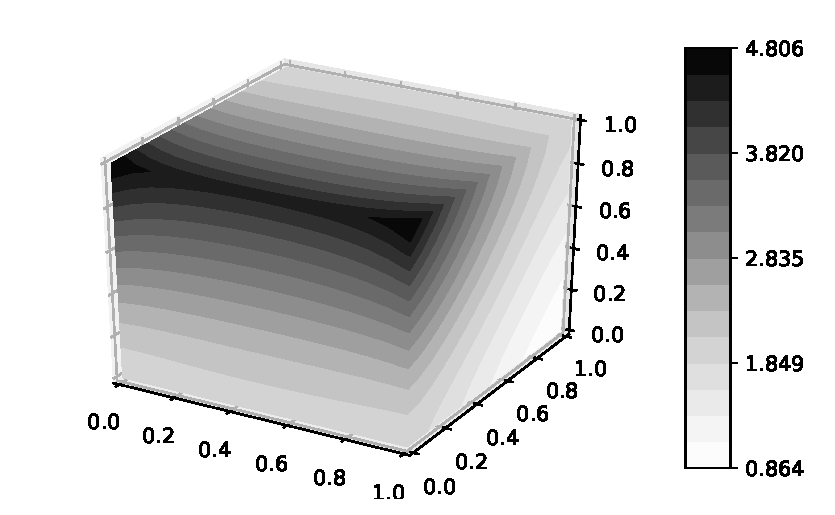
\includegraphics[width=1\linewidth]{boundary/theta_3d} \\ а) $\theta$
%        \end{minipage}
%        \hfill
%        \begin{minipage}[b][][b]{0.49\linewidth}
%            \centering
%            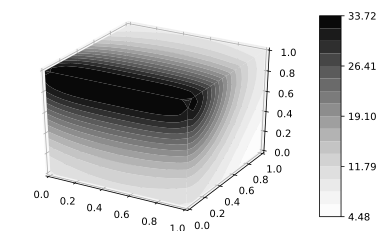
\includegraphics[width=1\linewidth]{boundary/phi_3d} \\ б) $\varphi$
%        \end{minipage}
%        \label{fig:4_1:boundary_3d}
%    \end{figure}
%\end{frame}
%\note{
%    Линеаризируем её методом Ньютона.
%    (Существенно улучшает сходимость алгоритмов!!
%    Что важно при решении задач типа Коши и др.)
%
%    Начальное приближение выберем нулевым.
%    Для нахождения состояния потребовалось шесть итераций,
%    результат представлен на рисунке.
%
%
%    Предложенный в работе алгоритм и программа решения краевых задач позволяет
%    уверенно рассчитывать температурное поле и поле излучения для произвольных областей.
%}
%
%\subsection{Квазистационарная модель}\label{subsec:qst}
%\begin{frame}
%    \frametitle{Квазистационарная модель}
%    \begin{align}
%        \frac{\partial\theta}{\partial t} - a\Delta\theta
%        + b\kappa_a (|\theta|\theta^3 - \phi) &= 0, \label{eq:1_5:1}\\
%        - \alpha\Delta\phi + \kappa_a (\phi - |\theta|\theta^3 ) &= 0,
%        \quad x \in \Omega, \quad 0 < t < T ; \label{eq:1_5:1+} \\
%        a \frac{\partial \theta}{\partial n}
%        +\left.\beta\left(\theta-\theta_{b}\right)\right|_{\Gamma}&=0,
%        \quad \alpha \frac{\partial \varphi}{\partial \mathbf{n}} + \gamma
%        (\varphi-\theta_b^4)|_{\Gamma} = 0 \text{ на } \Gamma; \label{eq:1_5:2} \\
%        \theta|_{t=0} &= \theta_0. \label{eq:1_5:3}
%    \end{align}
%    Предполагаем, что
%    \begin {itemize}
%        \item (j) $a, b, \alpha, \kappa_{a} =$ Const $>0$,
%        \item (jj) $\theta_{b}, q_{b}, u=\theta^4_b \in U, r
%        =a\left(\theta_{b}+q_{b}\right) \in L^{5}(\Sigma), \; \theta_{0} \in L^{5}(\Omega)$.
%    \end{itemize}
%
%    Здесь $\Sigma = \Gamma \times (0, T)$, $U$ -- пространство $L^{2}(\Sigma)$.
%
%    \begin{lemma}[1.20]
%        Пусть выполняются условия (j), (jj).
%        Тогда существует единственное слабое решение задачи~\eqref{eq:1_5:1}--\eqref{eq:1_5:3} и справедливо
%        \[
%            \psi=[\theta]^{5 / 2} \in L^{\infty}(0, T ; H) \cap L^{2}(0, T ; V),
%            \quad[\theta]^{4} \in L^{2}(0, T ; H).
%        \]
%    \end{lemma}
%\end{frame}
%\note{
%    Квазистационарная модель
%    Квазистационарная модель -- медленные изменения со временем или
%    имеющую относительно длительный период стабильности по сравнению с
%    интересующим масштабом времени.
%    Такие модели часто используются, когда
%    изучаемая система находится в равновесии или близка к нему, но при этом мо
%    жет испытывать небольшие, медленные колебания со временем.
%    Термин ‘квази‘ означает, что система не совсем стационарна,
%    ее состояние меняется настолько медленно,
%    его можно считать почти стационарным для определенных анализов или целей.
%
%    В контексте теплообмена, излучения или других физических процессов
%    квазистационарные модели могут использоваться для описания сценариев, ко
%    гда параметры и свойства системы меняются очень медленно по сравнению с
%    масштабом времени конкретного изучаемого явления.
%    Такие модели могут упростить анализ и снизить вычислительную сложность, позволяя исследователям
%    сосредоточиться на основных аспектах проблемы.
%
%    [Лемма] -- теоретический результат является новым и используется для обоснования
%    корректности оптимизационного метода для квазистационарной модели с данными Коши.
%}
%
%\subsection{Квазилинейная модель}\label{subsec:ql}
%\begin{frame}
%    \frametitle{Квазилинейная модель}
%    \begin{gather}
%        \sigma \partial \theta / \partial t
%        -\operatorname{div}(k(\theta) \nabla \theta)
%        +b\left(\theta^{3}|\theta|-\varphi\right)=f, \label{eq:1_6:1}\\
%        -\operatorname{div}(\alpha \nabla \varphi)
%        +\beta\left(\varphi-\theta^{3}|\theta|\right)=g, x \in \Omega, 0<t<T, \label{eq:1_6:2}\\
%        k(\theta) \partial_{n} \theta+\left.p\left(\theta-\theta_{b}\right)\right|_{\Gamma}=0,
%        \alpha \partial_{n} \varphi
%        +\left.\gamma\left(\varphi-\theta_{b}^{4}\right)\right|_{\Gamma}=0,
%        \left.\quad \theta\right|_{t=0}=\theta_{in}.\label{eq:1_6:3}
%    \end{gather}
%
%    Предполагаем, что:
%    \begin{itemize}
%        \item (k1) $\alpha, \beta, \sigma \in L^{\infty}(\Omega),
%        \quad b=r \beta, r = Const > 0; \alpha \geq \alpha_{0}, \beta \geq \beta_{0},
%        \sigma \geq \sigma_{0}, \alpha_{0}, \beta_{0}, \sigma_{0}=$ Const $>0$.
%
%        \item (k2) $0<k_{0} \leq k(s) \leq k_{1},\left|k^{\prime}(s)\right| \leq k_{2},
%        s \in \mathbb{R}, \quad k_{j}=$ Const.
%
%        \item (k3) $0 \leq \theta_{b} \in L^{\infty}(\Sigma), 0 \leq \theta_{\text{in}}
%        \in L^{\infty}(\Omega)$; $\gamma_{0} \leq \gamma \in L^{\infty}(\Gamma), p_{0}
%        \leq p \in L^{\infty}(\Gamma), \gamma_{0}, p_{0}=$ Const $>0$.
%
%        \item (k4) $0 \leq f, g \in L^{\infty}(Q).$
%    \end{itemize}
%
%
%    \begin{theorem}[1.7]
%        \label{th:1_6:1}
%        Если выполнены условия (k1)--(k4), то существует хотя бы одно
%        решение задачи~\eqref{eq:1_6:1}--\eqref{eq:1_6:3}.
%    \end{theorem}
%    \begin{theorem}[1.8]
%        Если выполнены условия (k1)--(k4) и $\theta_{*}, \varphi_{*}$ является
%        решением задачи~\eqref{eq:1_6:1}--\eqref{eq:1_6:3}
%        так, что $\theta_{*}, \nabla \theta_{*} \in L^{\infty}(Q)$,
%        то других ограниченных решений этой задачи нет.
%    \end{theorem}
%\end{frame}
%\note{
%    Зависимость коэффициента теплопроводности от температуры,
%    $\sigma$ – произведение удельной теплоемкости на объемную плотность (кг на м3),
%    f и g описывают вклад источников тепла и излучения соответственно.
%    Положительные параметры ... описывают радиационные и теплофизические свойства среды.
%
%    Свойства модели, установленные в этих теоремах являются новыми и
%    позволяют говорить о корректности квазилинейной модели.
%}
%
\section{Граничные обратные задачи и задачи с данными Коши}\label{sec:rev}

\subsection{Граничная обратная задача}\label{subsec:rev}
\begin{frame}
    \frametitle{Граничная обратная задача}
    Модель имеет следующий вид
    \begin{wrapfigure}{r}{0.3\textwidth}
        \centering{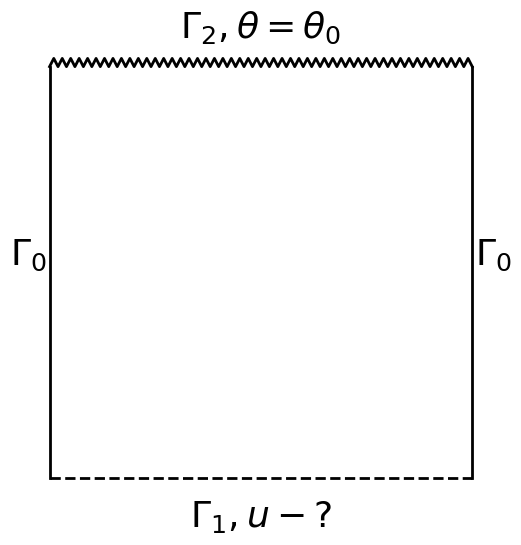
\includegraphics[width=1\linewidth]{omega_1}}
%        \caption*{$\Gamma \coloneqq \partial \Omega =\overline{\Gamma}_0 \cup \overline{\Gamma}_1 \cup \overline{\Gamma}_2$}
    \end{wrapfigure}
    \begin{gather}
        \label{eq:2_1:initial}
        - a \Delta \theta + b \kappa_a(\theta ^ 3 | \theta | - \varphi) = 0, \\
        - \alpha \Delta \varphi + \kappa_a (\varphi - \theta ^3 | \theta |) = 0,
    \end{gather}
    \begin{equation}
        \label{eq:2_1:initial-boundary}
        \begin{aligned}
            \Gamma &: \; a \partial_n \theta + \beta (\theta - \theta _b) = 0, \\
            \Gamma_0 \cup \Gamma_2 &: \; \alpha \partial_n \varphi
            + \gamma(\varphi - \theta_b ^4 ) = 0, \\
            \Gamma_1 &: \; \alpha \partial_n \varphi + u(\varphi - \theta_b ^4 ) = 0. \\
        \end{aligned}
    \end{equation}
    $\Gamma_0, \Gamma_1, \Gamma_2$ не имеют пересечений.

    Функции $\gamma, \theta_b, \beta$ известны.
    \textit{Неизвестная функция $u$ характеризует отражающие свойства участка границы $\Gamma_1$}.
    Предполагается, что $0 < u_1 \leq u \leq u_2$.

    \textbf{Обратная задача} заключается в отыскании тройки $\theta, \varphi, u$
    по дополнительному условию $\theta|_{\Gamma_2} = \theta_0$.

    \textbf{Экстремальная задача} заключается в минимизации функционала
    \begin{equation}
        \label{eq:2_1:quality}
        J(\theta) = \frac{1}{2} \int_{\Gamma_2} (\theta - \theta_0)^2 d\Gamma
    \end{equation}
    на решениях краевой задачи~\eqref{eq:2_1:initial}--\eqref{eq:2_1:initial-boundary}.
\end{frame}
\note{
    \begin{itemize}
        \item Первая из рассматриваемых задач представляется двумя уравнениями ...
        \item Пару $\theta, \varphi$ - будем называть состоянием системы.
        \item Дополняется граничными условиями ...
        \item Если же параметр отражательной способности неизвестен на части границы,но ...
        \item Неизвестные параметры среды мы будем называть функцией управления $u$.
        В данном случае, неизвестен параметр $\gamma$ на нижней границе.
        \item Краевая задача, где все параметры среды известны хорошо изучена, (АЮ 2015)
        \item Об обратной задаче нет данных - формулируем задачу опт. управления.
        \item Квазирешение и его существование.
    \end{itemize}
}


\begin{frame}
    \frametitle{Нахождение квазирешения обратной задачи}
    \begin{gather}
        A_1 \theta + b \kappa_a (| \theta | \theta^3 - \varphi) =
        f, A_2 \varphi + \kappa_a (\varphi - |\theta|\theta^3) + F(\varphi, u) = g.
        \label{eq:2_1:weakOperational}\\
        J(\theta) = \frac{1}{2} \int_{\Gamma_2} (\theta - \theta_0)^2 d\Gamma,
        \label{eq:2_1:qualityOperational}\\
        A_1 p_1 + 4 |\hat{\theta}|^3 \kappa_a(b p_1 - p_2) = f_c,
        \;\; (f_c,v) = - \int_{\Gamma_2} (\hat{\theta} - \theta_0) v d\Gamma,
        \label{eq:2_1:theorem_2_eq1}\\
        A_2 p_2 + \kappa_a (p_2-b p_1) = g_c(p_2, \hat{u}),
        \;(g_c(p_2, \hat{u}), v) = -\int_{\Gamma_1} \hat{u} p_2 v d\Gamma,
        \label{eq:2_1:theorem_2_eq2}\\
        \int_{\Gamma_1} p_2 (\hat{\varphi} - \theta_b^4)(u-w) d\Gamma
        \leq 0 \quad \forall w \in U_{ad}. \label{eq:2_1:theorem_2_eq3}
    \end{gather}
    \textbf{Алгоритм градиентного спуска с проекцией}
    \begin{enumerate}
        \item Выбор шага $\lambda$, числа итераций $N$, управления $u_0 \in U_{ad}$
        -- пространство допустимых управлений.
        \item для $k \leftarrow 0,1,2, \ldots, N$ выполнить:
        \begin{itemize}
            \item Для $u_{k}$, вычислить $y_k = \{\theta_k, \varphi_k\}$ из~\eqref{eq:2_1:weakOperational}.
            \item Вычислить значение $J(\theta_k)$ из уравнения~\eqref{eq:2_1:quality}.
            \item Рассчитать $p_k=\{p_{1k},p_{2k}\}$
            из~\eqref{eq:2_1:theorem_2_eq1}--\eqref{eq:2_1:theorem_2_eq2},
            \item Пересчитать управление
            $u_{k+1} = P_{ad}\left[ u_k - \lambda (\varphi_k - \theta_b^4)p_{2k} \right]$.
        \end{itemize}
    \end{enumerate}
\end{frame}
\note{
    Предложенный в работе алгоритм поиска квазирешения обратной задачи основан
    на выведенных условиях оптимальности
    (доказано, что квазирешение должно
    удовлетворять~\eqref{eq:2_1:weakOperational}--\eqref{eq:2_1:theorem_2_eq2}),
    куда входят сопряженные функции для температуры $p_1$ и излучения $p_2$,
    а также связь между сопряженным состоянием и искомым граничным управлением.
    Для компактной записи краевых задач, используется современная операторная форма.
    Система~\eqref{eq:2_1:weakOperational} является операторной записью краевой задачи,
    где $A_{1,2}$ описывают диффузионные члены модели, остальные моделируют граничные условия.
    Уравнения~\eqref{eq:2_1:theorem_2_eq1}--\eqref{eq:2_1:theorem_2_eq2}
    это сопряженная система,
    а вариационное неравенство~\eqref{eq:2_1:theorem_2_eq3}
    устанавливает связь с оптимальным управлением.

    Приведём алгоритм градиентного спуска с проекцией.
    Обратим внимание, что оператор проекции нужен
    из-за начальных ограничений на функцию управления
    (вызванных физичностью параметра, например).

    Отметим, что в силу невыпуклости экстремальной задачи градиентные алгоритмы не обладают
    свойством глобальной сходимости, что служит основой для их критики, зачастую заслуженной.

    Однако свойства диффузионных моделей сложного теплообмена представленные в диссертации
    и правильный выбор шага градиентного метода обеспечивают сходимость для
    рассматриваемых задач.
    Следующие примеры этот факт демонстрируют.
}

\begin{frame}
    \textbf{Численные эксперименты:}

    \begin{wrapfigure}{r}{0.3\textwidth}
        \centering{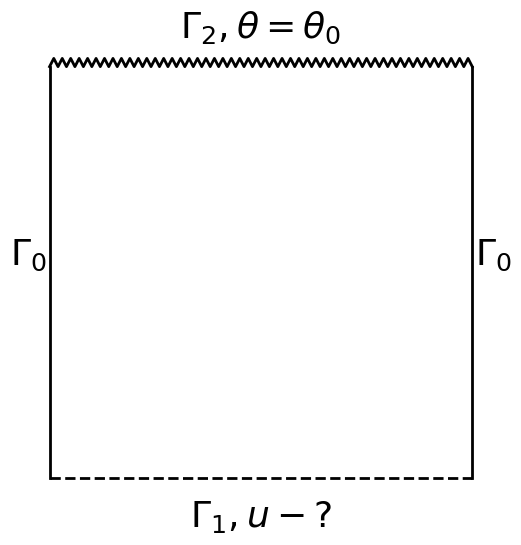
\includegraphics[width=1\linewidth]{omega_1}}
%        \caption*{$\Gamma \coloneqq \partial \Omega =\overline{\Gamma}_0 \cup \overline{\Gamma}_1 \cup \overline{\Gamma}_2$}
    \end{wrapfigure}
    Положим $\Omega = \{(x,y), 0 \leq x,y \leq 1\}$, $l = 1$ см.
    Граница $\partial\Omega$:
    \[
        \begin{aligned}
            \Gamma_0 & = \{x=\{0,1\}, y \in [0,1]\} \\
            \Gamma_1 & = \{x\in [0,1], y=0\}
            - \text{участок с неизвестными отр. свойствами}, \\
            \Gamma_2 & = \{x \in [0,1], y=1\} - \text{участок наблюдения}.
        \end{aligned}
    \]
    Будем также далее считать, что $a = 0.006[\text{см}^2/\text{c}]$,
    $b=0.025[\text{см}/\text{с}]$, $\beta = 0.00005[\text{см}/\text{с}]$,
    $\kappa=1[\text{см}^{-1}]$, $\kappa_s = 0$, $A = 0$, $\gamma = 0.3$.
    Температуру на границе $\Omega$ положим равной $\theta_b = (x^2+y^2)/3$.

    При указанных параметрах для первого эксперимента выберем следующее тестовое
    значение функции $u$:
    \begin{equation*}
        u(x)=
        \begin{cases}
            0.01, & \text{если } x \le 0.5, \\
            0.5, & \text{если } x > 0.5,
        \end{cases}
    \end{equation*}
    и для второго эксперимента:
    $u(x)=0.49x+0.01$.
\end{frame}
\note{
    Положим параметры среды, соответствующие стеклу и зададим тестовую функцию управления
    как показано на слайде.
    Пластинка, у которого боковые стороны "обычные", верхняя грань - участок наблюдения,
    нижняя грань - участок под "контролем".
}


\begin{frame}
    \textbf{Результаты моделирования:}

    \centering
    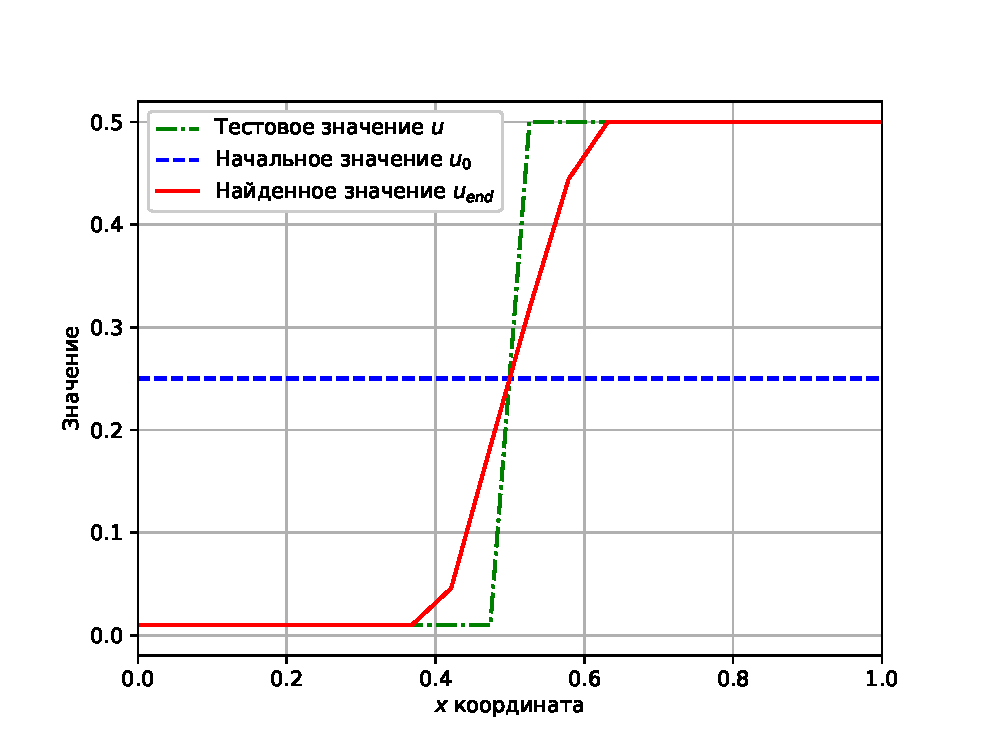
\includegraphics[width=0.42\linewidth]{dvmg368/1}
    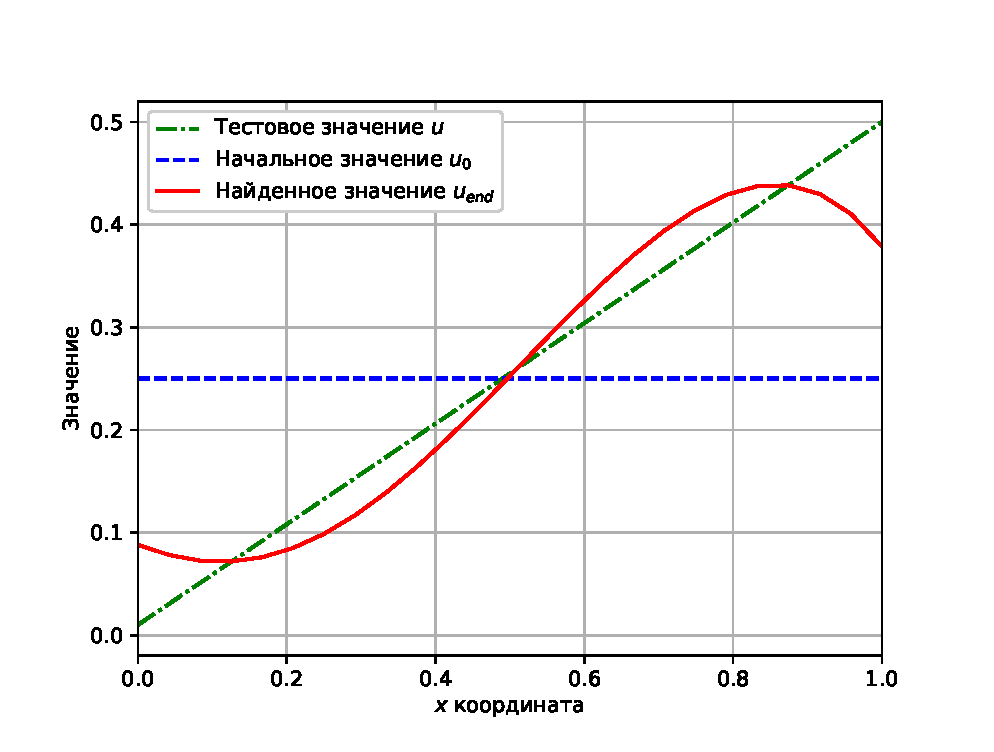
\includegraphics[width=0.42\linewidth]{dvmg368/2}
    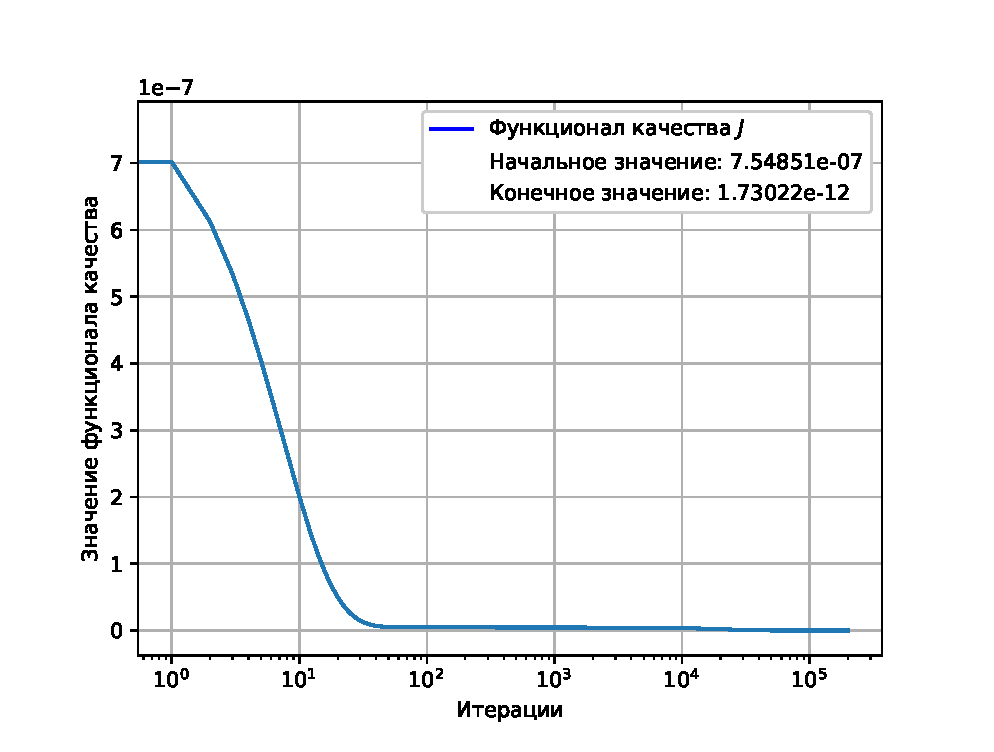
\includegraphics[width=0.42\linewidth]{dvmg368/3}
    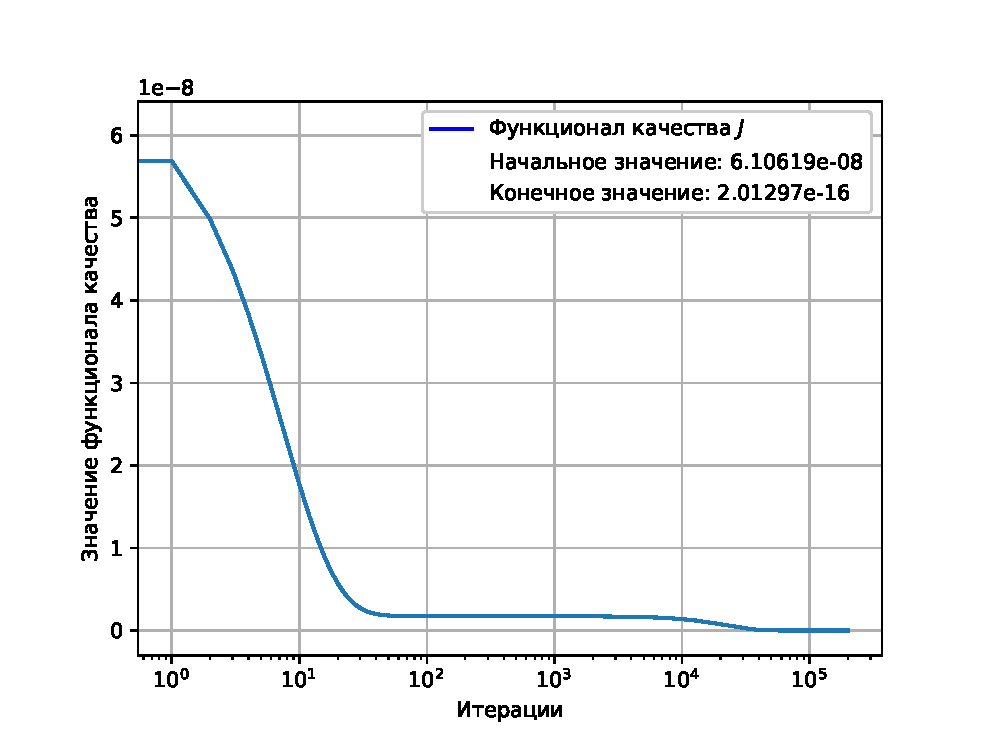
\includegraphics[width=0.42\linewidth]{dvmg368/4}
\end{frame}
\note{
    Интересный эффект "среднего значения". Большое количество итераций.
    Обратить внимание на функционал качества.
    Для получения представленных результатов, использовался разработанный мной комплекс программ,
    включающий решение прямой задачи, сопряженной системы и алгоритм градиентного спуска.
}

\subsection{Обратная задача с условиями типа Коши}\label{subsec:rev_koshi}
\begin{frame}
    \frametitle{Задача без краевых условий для интенсивности излучения}
    \textbf{Краевая задача:}
    \begin{equation}
        \label{eq:2_2:eq1}
        - a \Delta \theta + b \kappa_a(\theta ^ 3 | \theta | - \varphi) = 0,  \quad
        - \alpha \Delta \varphi + \kappa_a (\varphi - \theta ^3 | \theta |) = 0,
    \end{equation}
    На $\Gamma$ известно температурное поле и тепловой поток:
    \begin{equation}
        \label{eq:2_2:bc2} \theta = \theta_b, \quad \partial_n\theta = q_b.
    \end{equation}
    Заменяем на <<искусственные>> краевые условия
    \begin{equation}
        \label{eq:2_2:bc3}
        a(\partial_n\theta+\theta) = r,\;\;
        \alpha(\partial_n\varphi+\varphi) = u \text{ на }\Gamma.
    \end{equation}
    Функция $r(x),\, x\in\Gamma$ является заданной, функция $u(x),\, x\in\Gamma$
    описывающая излучающие свойства участка границы, неизвестна.
    Получаем \textbf{обратную задачу}.

    \textbf{Задача оптимального управления} заключается в отыскании тройки
    $\{\theta_\lambda,\varphi_\lambda,u_\lambda\}$ такой, что
    \begin{equation}
        \label{eq:2_2:cost}
        J_\lambda(\theta, u) = \frac{1}{2}\int\limits_\Gamma (\theta - \theta_b)^2 d\Gamma
        + \frac{\lambda}{2}\int\limits_\Gamma u^2 d\Gamma \rightarrow\inf
    \end{equation}
    на решениях краевой задачи, функция $u(x) x \in \Gamma$ играет роль управления.

    \begin{itemize}
        \item $(j) \;\; a,b,\alpha,\kappa_a, \lambda ={\textrm Const}> 0,$
        \item $(jj) \;\, \theta_b, \,q_b \in U,\;\; r=a(\theta_b+q_b)$.
    \end{itemize}
    \begin{theorem}[2.5]
        \label{th:2_2:3}
        Пусть выполняются условия $(j),(jj)$ и существует решение
        задачи~\eqref{eq:2_2:eq1}--\eqref{eq:2_2:bc2}.
        Если $\{\theta_\lambda,\varphi_\lambda,u_\lambda\}$ -- решение
        задачи оптимального управления для $\lambda>0$, то существует последовательность $\lambda\to +0$
        такая, что
        $\theta_\lambda\rightarrow\theta_*, \;\; \varphi_\lambda\rightarrow\varphi_*
        \text{ слабо в }V,\text{ сильно в }H$,
        где $\theta_*,\varphi_*$ -- решение задачи~\eqref{eq:2_2:eq1}--\eqref{eq:2_2:bc2}.
    \end{theorem}
\end{frame}
\note{
    23. Не задано $\varphi$!
    В основе разработанного алгоритма решения лежит анализ экстремальной задачи.

    Строго обосновано существование решения экстр задачи.
    Кроме того, и это принципиально важно, показана сходимость решений экстремальных задач
    к решению задачи~\eqref{eq:2_2:eq1}--\eqref{eq:2_2:eq2}
    без краевых условий для интенс излучения при $\lambda$ стремящемся к 0.
}
\begin{frame}
    \textbf{Разрешимость задачи оптимального управления и условия оптимальности}

    \begin{theorem}[2.3]
        \label{th:2_2:1}
        Пусть выполняются условия $(j), (jj)$.
        Тогда существует решение задачи $CP$.
    \end{theorem}
    \begin{theorem}[2.4]
        \label{th:2_2:2}
        Пусть выполняются условия $(j),(jj)$.
        Если $\{\hat{\theta}, \hat{\varphi}, \hat{u}\}$ -- решение задачи оптимального управления,
        то существует единственная пара $\{p_1, p_2 \} \in V\times V$ такая, что
        \begin{equation}
            \label{eq:2_2:as}
            aAp_1 +4|\hat{\theta}|^3 \kappa_a(bp_1 - p_2) = B(\theta_b - \hat{\theta}), \;\;
            \alpha A p_2 + \kappa_a (p_2 - b p_1)=0
        \end{equation}
        и при этом $\lambda\hat{u} = p_2$.
    \end{theorem}


    \textbf{Алгоритм решения задачи без краевых условий для интенсивности излучения}

    1.\ Выбираем значение градиентного шага $\varepsilon$,

    2.\ Выбираем количество итераций $N$,

    3.\ Выбираем начальное приближение для управления $u_{0} \in U$,

    4.\ для $k \leftarrow 0,1,2, \ldots, N$ выполнить:

    \hspace{1cm} a.\ Для заданного $u_{k}$, вычислить состояние
    $y_{k}=\left\{\theta_{k}, \varphi_{k}\right\}$, решение
    задачи~\eqref{eq:2_2:eq1}--\eqref{eq:2_2:bc1}.

    \hspace{1cm} b.\ Вычислить значение функционала качества
    $J_{\lambda}\left(\theta_{k}, u_{k}\right)$.

    \hspace{1cm} c.\ Из уравнений~\eqref{eq:2_2:as}, вычислить сопряженное
    состояние $p_{k}=\left\{p_{1k}, p_{2k}\right\}$,
    где $\widehat{\theta} \coloneqq \theta_{k}, \widehat{u} \coloneqq u_{k}$.

    \hspace{1cm} d.\ Пересчитать управление
    $u_{k+1}=u_{k}-\varepsilon\left(\lambda u_{k}-p_{2}\right)$.


    Значение параметра $\varepsilon$ выбирается эмпирически.
    Количество итераций $N$ выбирается достаточным для выполнения условия
    $J_\lambda(\theta_k, u_k) - J_\lambda(\theta_{k+1}, u_{k+1}) < \delta$, где $\delta>0$
    определяет точность расчетов.
\end{frame}
\note{
    25. Условия оптимальности лежат в основе численного метода
}

\begin{frame}
    \textbf{Пример 1.}
    Приведем примеры расчетов для куба $\Omega = {(x, y, z), 0 \leq x,y,z \leq l}$.

    Будем считать, что $l=1~\text{см}$, $a = 0.006[\text{см}^2/\text{c}]$,
    $b=0.025[\text{см}/\text{с}]$, $\kappa_a=1[\text{см}^{-1}]$, $\alpha = 0.(3)[\text{см}]$.
    Параметр регуляризации $\lambda=10^{-12}$.

    Определим $r$ и $u$ в~\eqref{eq:2_2:bc3} как $r = 0.7, \quad u = \hat u = 0.5$.
    Для обозначенных параметров рассчитаем функции $\theta$, $\varphi$ из решения граничной задачи
    и положим $\theta_b = \theta|_\Gamma$.
    Нормальная производная $\partial_n \theta = q_b = r / a - \theta_b$.

    Применяя алгоритм градиентного спуска найдем решение задачи оптимального управления.
    \begin{figure}[h!t]
        \begin{minipage}[b][][b]{0.49\linewidth}
            \centering
            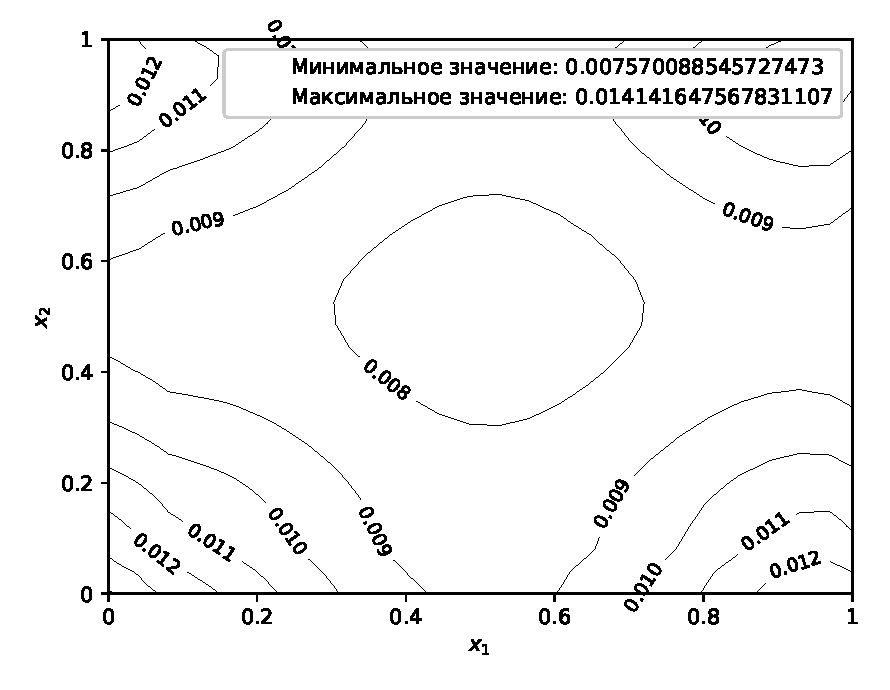
\includegraphics[width=1\linewidth]{jvm-2020/exp1/theta_n_diff_iso}
            \\ а) $|\partial_n\theta_\lambda-q_b|/|q_b|$
        \end{minipage}
        \hfill
        \begin{minipage}[b][][b]{0.49\linewidth}
            \centering
            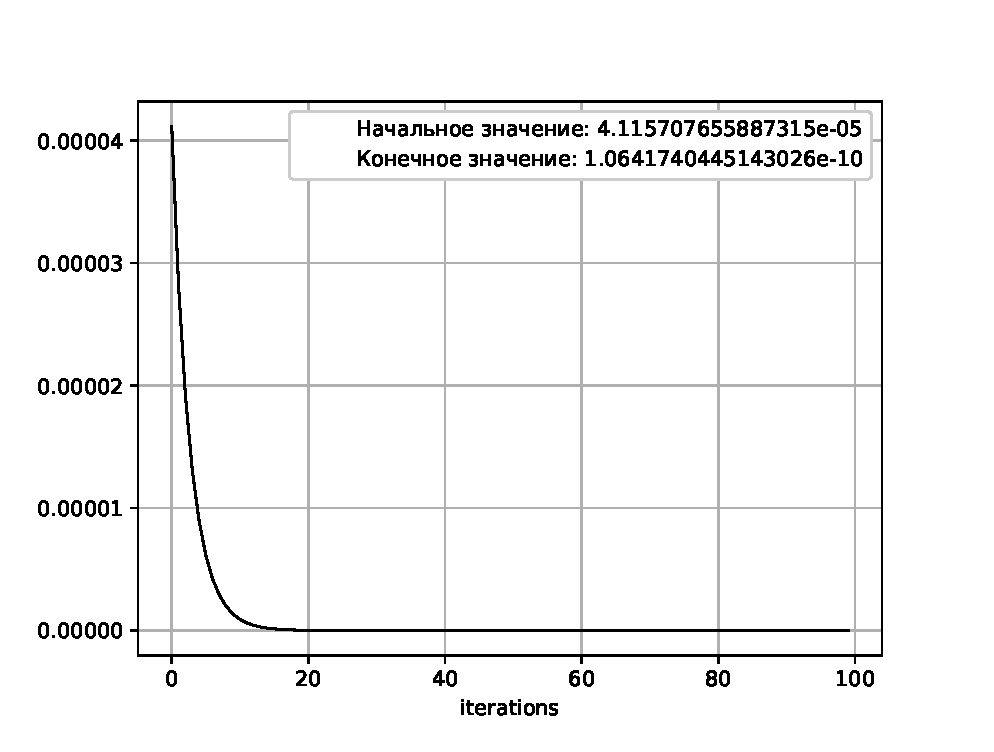
\includegraphics[width=1\linewidth]{jvm-2020/exp1/quality}
            \\ б) Значение функционала качества
        \end{minipage}
        \label{fig:4_4:0}
    \end{figure}
\end{frame}
\note{
    Обратите внимание на малость функционала качества.
    Сравним с тем, что получилось -- довольно близко, но не идеально.
    Уменьшение параметра регуляризации повышает точность решения,
    но и увеличивает вычислительные затраты.
}

\begin{frame}
    \textbf{Пример 2.}


    Зададим функции $\theta_{b}, q_{b}$ в краевом условии~\eqref{eq:2_2:bc2}
    следующим образом:
    \[
        \theta_{b}=0.1 z+0.3, \quad q_{b}=
        \begin{cases}
            0.11, & \text { если } z=1, \\
            0, & \text { если } 0<z<1, \\
            -0.15, & \text { если } z=0.
        \end{cases}
    \]

    В данном примере оптимальное управление $u$ в качестве тестового не задается.
    Начальное значение функционала качества $J_\lambda$ составляет $7.20 \cdot 10^{-6}$.
    Финальное значение $2.86 \cdot 10^{-10}$.

    \begin{figure}[h!t]
        \begin{minipage}[b][][b]{0.49\linewidth}
            \centering
            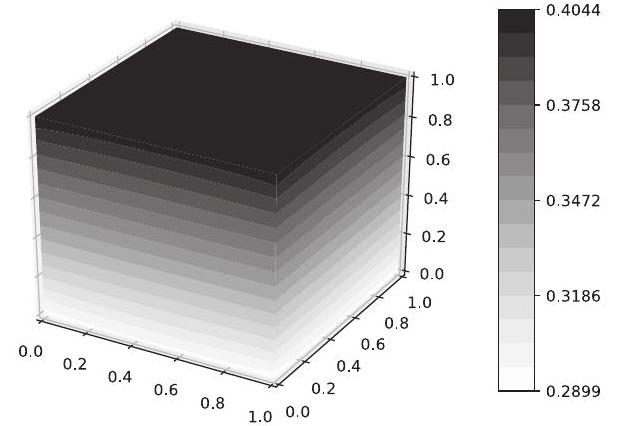
\includegraphics[width=0.9\linewidth]{jvm-2020/dvmg/3b}
            \\ а) Полученное температурное поле $\theta_\lambda$
        \end{minipage}
        \hfill
        \begin{minipage}[b][][b]{0.49\linewidth}
            \centering
            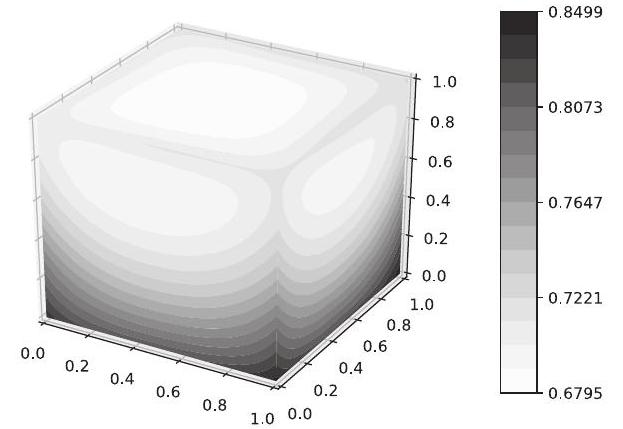
\includegraphics[width=1\linewidth]{jvm-2020/dvmg/2a}
            \\ б) Полученное поле излучения $\varphi_\lambda$
        \end{minipage}
        \label{fig:4_4:3}
    \end{figure}

\end{frame}
\note{
    "Честный" эксперимент - используем то, что полагается в исходной задаче.
    Функционал качества (его динамика) позволяет предположить аналогичный порядок
    близости (с предыдущим примером)
    точного и аппроксимированного решений.
    Обратите внимание на линейность $\theta_b$ по оси $z$.
}


\subsection{Квазистационарная задача с данными Коши}\label{subsec:qst_koshi}
\begin{frame}
    \frametitle{Квазистационарная модель с данными Коши}
    \textbf{Начально-краевая задача:}
    \begin{equation}
        \label{eq:2_3:1}
        \begin{split}
            & \frac{\partial \theta}{\partial t} - a \Delta \theta
            + b \kappa_{a} \left(|\theta| \theta^{3}-\varphi\right) = 0,\\
            & - \alpha \Delta \varphi
            + \kappa_{a} \left(\varphi-|\theta| \theta^{3}\right) = 0,
            \quad x \in \Omega, \quad 0 < t < T;
        \end{split}
    \end{equation}
    \begin{align}
        a \left(\partial_{n} \theta+\theta\right)=r,
        & \quad \alpha\left(\partial_{n} \varphi
        + \varphi\right) = u \text { на } \Gamma;  \label{eq:2_3:2}\\
        & \left.\theta\right|_{t=0} = \theta_{0}. \label{eq:2_3:3}
    \end{align}


    \textbf{Экстремальная задача} состоит в том, чтобы найти тройку
    $\left\{\theta_{\lambda}, \varphi_{\lambda}, u_{\lambda}\right\}$ такую, что
    \begin{equation}
        \label{eq:2_3:4}
        J_{\lambda}(\theta, u)=\frac{1}{2} \int_{0}^{T}
        \int_{\Gamma}\left(\theta-\theta_{b}\right)^{2} d \Gamma d t+\frac{\lambda}{2}
        \int_{0}^{T} \int_{\Gamma} u^{2} d \Gamma d t \rightarrow \inf
    \end{equation}
    на решениях задачи~\eqref{eq:2_3:1}--\eqref{eq:2_3:3}.
    \begin{itemize}
        \item $(k)\; a, b, \alpha, \kappa_{a}, \lambda=$ Const $>0$,
        \item $(kk)\; \theta_{b}, q_{b} \in U, r=a\left(\theta_{b}+q_{b}\right)
        \in L^{5}(\Sigma), \; \theta_{0} \in L^{5}(\Omega)$.
    \end{itemize}


    \begin{theorem}[2.8]
        \label{th:2_3:3}
        Пусть выполняются условия $(k), (kk)$ и существует решение
        $\theta, \varphi \in$ $L^{2}\left(0, T ; H^{2}(\Omega) \right)$
        задачи~\eqref{eq:2_3:1}--\eqref{eq:2_3:3}.
        Если $\left\{\theta_{\lambda}, \varphi_{\lambda}, u_{\lambda}\right\}$
        — решение задачи $OC$ при $\lambda>0$, то при $\lambda\rightarrow+0$
        \[
            \begin{gathered}
                \theta_{\lambda} \rightarrow \theta \text { слабо в } L^{2}(0, T ; V),
                \text { сильно в } L^{2}(Q), \\
                \varphi_{\lambda} \rightarrow \varphi \text { слабо в } L^{2}(0, T ; V).
            \end{gathered}
        \]
    \end{theorem}
\end{frame}
\note{
    27. Аналог стационарной задачи с небольшими сдвигами по времени.
    Для оптимизационного метода решения задачи требуются результаты анализа кв.стц. модели из гл. 1!
    параметр u неизвестен.
}

\begin{frame}
    Область $\Omega \times(-L, L)$,
    где $\Omega=$ $\left\{x=\left(x_{1}, x_{2}\right): 0<x_{1,2}<d\right\}$.


    Определим параметры:
    $d=1(\text{м})$, $a=0.9210^{-4}(\text{м}^{2} / \text{с})$,
    $b=0.19(\text{м} / \text{с})$, $\alpha=0.0333(\text{м})$,
    $\kappa_{a}=1\left(\text{м}^{-1}\right)$, $T = 1(\text{c})$.
    \begin{figure}[h!t]
        \begin{minipage}[b][][b]{0.49\linewidth}
            \centering
            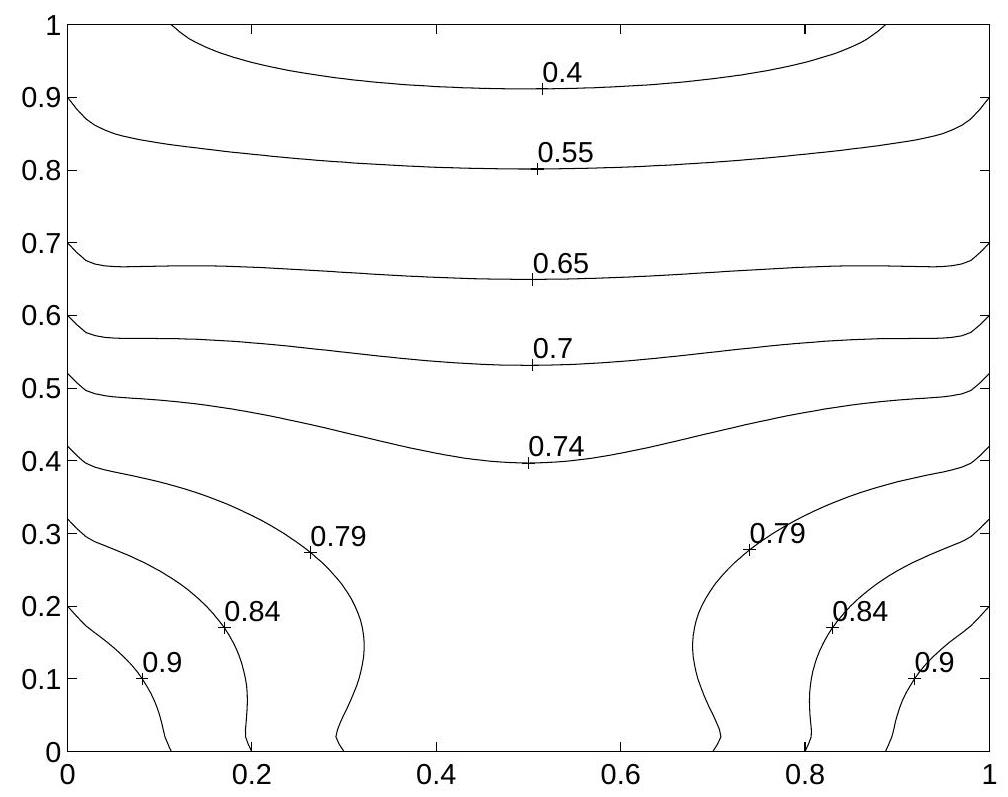
\includegraphics[width=1\linewidth]{paper03/1} \\ а) Поле температуры,
            полученное в статье *
        \end{minipage}
        \hfill
        \begin{minipage}[b][][b]{0.49\linewidth}
            \centering
            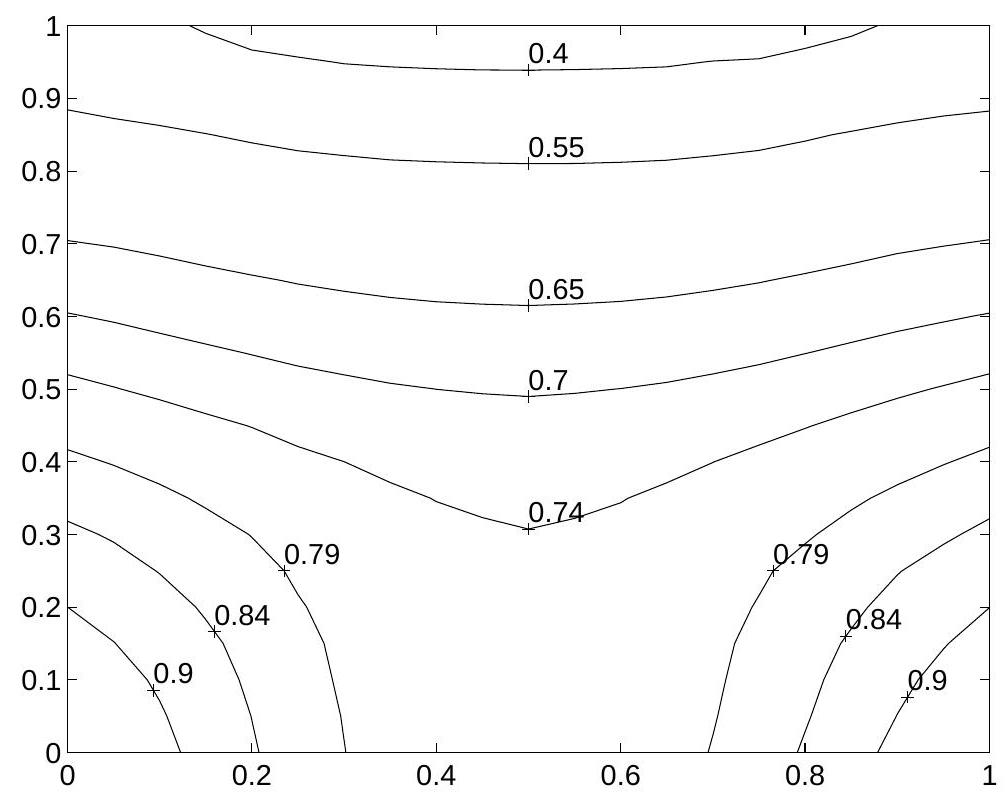
\includegraphics[width=1\linewidth]{paper03/2} \\
            б) Поле температуры, полученное предложенным алгоритмом
        \end{minipage}
        \label{fig:4_3:1}
    \end{figure}
    \tiny{* A. Y. Chebotarev, A. E. Kovtanyuk и N. D. Botkin. — \textit{«Problem of
    radiation heat exchange with boundary conditions of the Cauchy type»}. —
    Communications in Nonlinear Science and Numerical Simulation 75 (2019),
        с. 262—269.}
\end{frame}
\note{

    52. Приведены изображения сравнения полученных результатов в рамках работы
    над диссертацией и коллег из Мюнхена (финальный момент времени)
    Параметры среды соответствуют воздуху при нормальном атмосферном давлении и температуре 400C.


    N.Botkin для расчетов использовал, разработанную в TUM программу, использующую
    эрмитов прямоугольный (конформный) элемент Богнера-Фокса-Шмидта и сведение задачи к нестационарной.
    Не ясно, что же такое случилось с пространством решений,
    что потребовались столь экзотические конечные элементы.

    Фактически ему пришлось решать краевую задачу для нелинейного уравнения 4 порядка.
    Предложенный в работе оптимизационный алгоритм является более простым и дает фактически те же результаты.
    Использовались конечные элементы Галёркина (Лагранжа-1).

}

\subsection{Стационарная задача с условиями Коши на части границы}\label{subsec:st-koshi}
\begin{frame}
    \frametitle{Стац.\ задача с условиями Коши для температуры на части границы}
    \begin{wrapfigure}{r}{0.4\textwidth}
        \centering{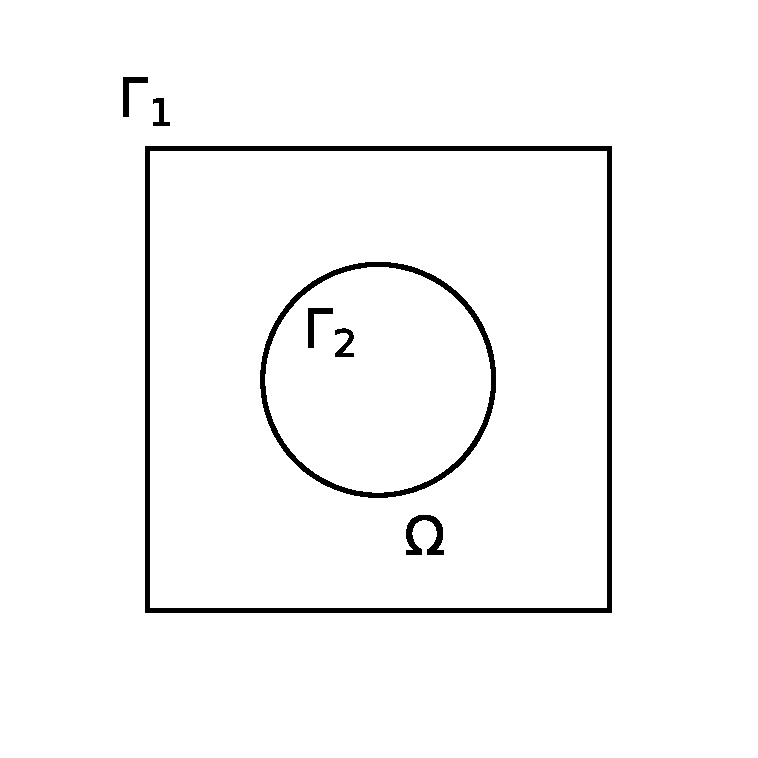
\includegraphics[width=1\linewidth]{omega-circle}}
%        \caption*{$\Gamma \coloneqq \partial \Omega =\overline{\Gamma}_0 \cup \overline{\Gamma}_1 \cup \overline{\Gamma}_2$}
    \end{wrapfigure}
    Рассмотрим область $\Omega$ с границей $\Gamma=\partial\Omega$.
    \begin{gather}
        \label{eq:2_4:eq1}
        - a\Delta\theta + b\kappa_a(\theta^4 - \varphi) = 0,   \\
        -\alpha \Delta \varphi + \kappa_a(\varphi- \theta^4) = 0.
    \end{gather}
    $\Gamma \coloneqq \partial \Omega =\overline{\Gamma}_1 \cup \overline{\Gamma}_2$
    так, что $\Gamma_1 \cap \Gamma_2 =  \emptyset$.
    На всей границе $\Gamma$ задается тепловой поток $q_b$,
    \begin{equation}
        \label{eq:2_4:bc1}
        a\partial_n\theta = q_b, \quad x\in \Gamma.
    \end{equation}
    Для задания краевого условия для интенсивности излучения требуется знать функцию $\gamma$.
    В случае, если эта функция неизвестна на части границы $\Gamma_2$,
    краевое условие для интенсивности излучения на $\Gamma_2$ не ставится, а в качестве условия
    переопределения на $\Gamma_1$, в дополнение к условию на
    $\varphi$, задается температурное поле $\theta_b$,
    \begin{equation}
        \label{eq:2_4:bc2}
        \alpha\partial_n\varphi + \gamma (\varphi - \theta_{out} ^4 ) = 0,\;
        \theta=\theta_b\quad \text{ на } \Gamma_1.
    \end{equation}.

\end{frame}
\note{
    30. Рассмотрим случай если на всей границе известен поток, а параметр из гранич. условия
    для $\varphi$ неизвестен. Мы дополняем "доступный" участок информацией о температуре: $theta_b$.
    Если данные Коши заданы на части границы задача является ещё более сложной.
    Для точной постановки нет результатов по её корректности.
    Однако предлагаемый далее оптимизационный метод полностью теоретически обоснован и
    лежит в основе соответствующего программного комплекса для численного решения.
}

\begin{frame}
    \textbf{Постановка задачи управления}


    Введем новую неизвестную функцию
    $\psi= a\theta + \alpha b \varphi$.

    \textbf{Краевая задача}:
    \begin{equation}
        \label{eq:2_4:eq2}
        - a \Delta \theta + g (\theta) = \frac{\kappa_a}{\alpha}\psi, \quad
        \Delta \psi = 0, \; x \in \Omega,
    \end{equation}
    \begin{equation}
        \label{eq:2_4:bc3}
        a \partial_n \theta = q_b \; \text{ на }\Gamma, \;\;
        \alpha \partial_n \psi + \gamma \psi  =  r,\;\;
        \theta = \theta_b  \text{ на }\Gamma_1.
    \end{equation}
    Здесь $g(\theta) = b \kappa_a|\theta|\theta^3 + \frac{a\kappa_a}{\alpha}\theta$, $r=\alpha b \gamma \theta_{out}^4+ \alpha q_b + a \gamma \theta_b$.


    Задача \textbf{оптимального управления}, аппроксимирующая краевую задачу,
    заключается в отыскании тройки $\{\theta_\lambda,\psi_\lambda,u_\lambda\}$ такой, что
    \begin{gather}
        \label{eq:2_4:cost}
        J_\lambda(\theta, u) =
        \frac{1}{2} \int \limits_{\Gamma_1} (\theta - \theta_b)^2 d \Gamma
        + \frac{\lambda}{2}\int\limits_{\Gamma_2} u^2 d\Gamma \rightarrow \inf, \\
        - a \Delta \theta + g (\theta) = \frac{\kappa}{\alpha}\psi, \quad
        \Delta \psi = 0, \; x \in \Omega, \\
        a \partial_n \theta + s \theta = q_b + s \theta_b,
        \; \alpha \partial_n \psi + \gamma \psi = r
        \text{ на } \Gamma_1,\\
        a \partial_n \theta = q_b, \;
        \alpha \partial_n \psi = u \text{ на } \Gamma_2.
    \end{gather}
    $\lambda, s > 0$ -- регуляризирующие параметры.


    \begin{itemize}
        \item $(l) \; a,b,\alpha,\kappa_a, \lambda, s ={\textrm Const}> 0.$
        \item $(ll) \; 0<\gamma_0\leq \gamma \in L^\infty(\Gamma_1), \; \theta_b, r \in L^2(\Gamma_1),\; q_b\in L^2(\Gamma)$.
    \end{itemize}

    \begin{theorem}[2.9]
        \label{th:2_4:1}
        При выполнении условий $(l), (ll)$ существует решение задачи оптимального управления.
    \end{theorem}

\end{frame}
\note{
    31. Используя замену, представленную на слайде, мы заменим исходную задачу, на краевую задачу
    с функциями $\theta$, $\psi$.
    Вместо системы двух нелинейных уравнений одно уравнение стало линейным (для $\Psi$)
    (!!!Где нелинейность в исходной задаче!!!)
    Два нелинейных заменили на нелинейное и линейное (пси - гармоническая, к тому же).
    Особо обратим внимание на параметр s, который пришлось добавить в данную постановку из-за
    того, что реализованный алгоритм не сходился. (Потеря точности решения.?)

    Расчёты выполнены при лямбда равной нулю.
}

\begin{frame}
    Рассмотрим двумерный случай:

    Квадрат $S = \{(x, y), 0 \leq x,y,z \leq 1~\text{см.}\}$ с
    круговой полостью $R$ с центром $b_0 =\{0.5, 0.5\}$
    $R = \{r, \| r - b_0 \| \leq 0.15~\text{см.} \}$.

    Рассматриваемая область $\Omega = S \setminus R$.
    $\Gamma \equiv \partial \Omega = \partial C \cup \partial B$, при этом
    $ \Gamma_2 = \partial R, \Gamma_1 = \partial S \setminus \Gamma_2$.
    Граничные данные $q_b$ и $\theta_b$ положим равными
    $
    \theta_b = 0.5, \;
    q_b =
    \begin{cases}
        0.2, & \text{если } x \in \Gamma_1 \\
        -0.2, & \text{если } x \in \Gamma_2.
    \end{cases}
    $
    \begin{figure}[h!t]
        \begin{minipage}[b][][b]{0.49\linewidth}
            \centering
            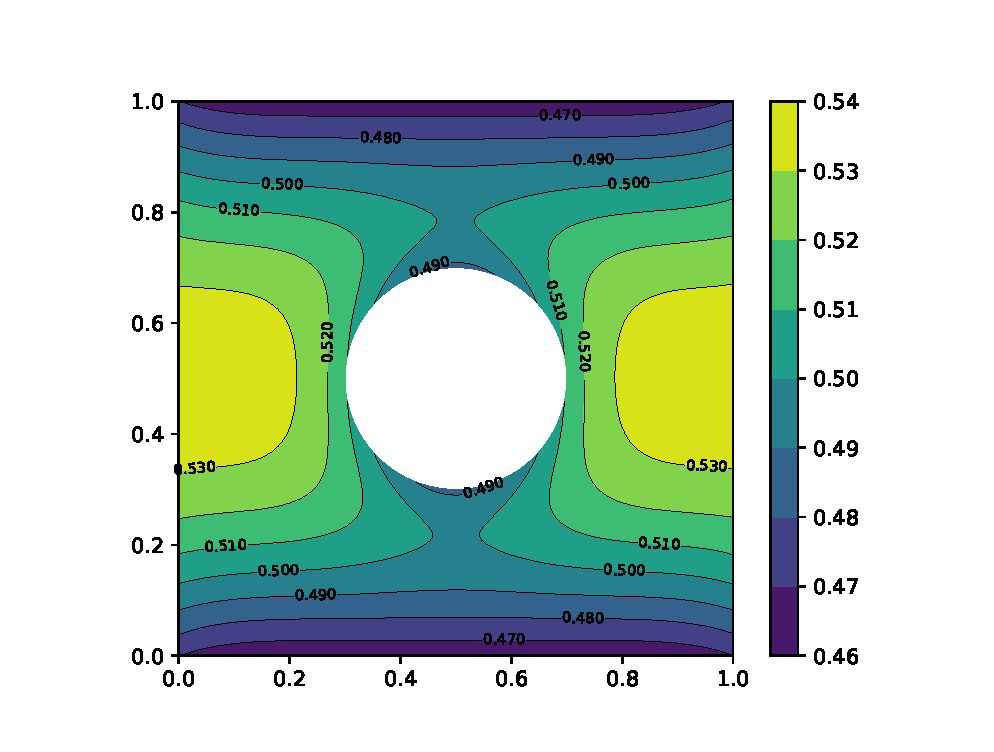
\includegraphics[width=1\linewidth]{theta_endf}
            \\ а) $\theta$
        \end{minipage}
        \hfill
        \begin{minipage}[b][][b]{0.49\linewidth}
            \centering
            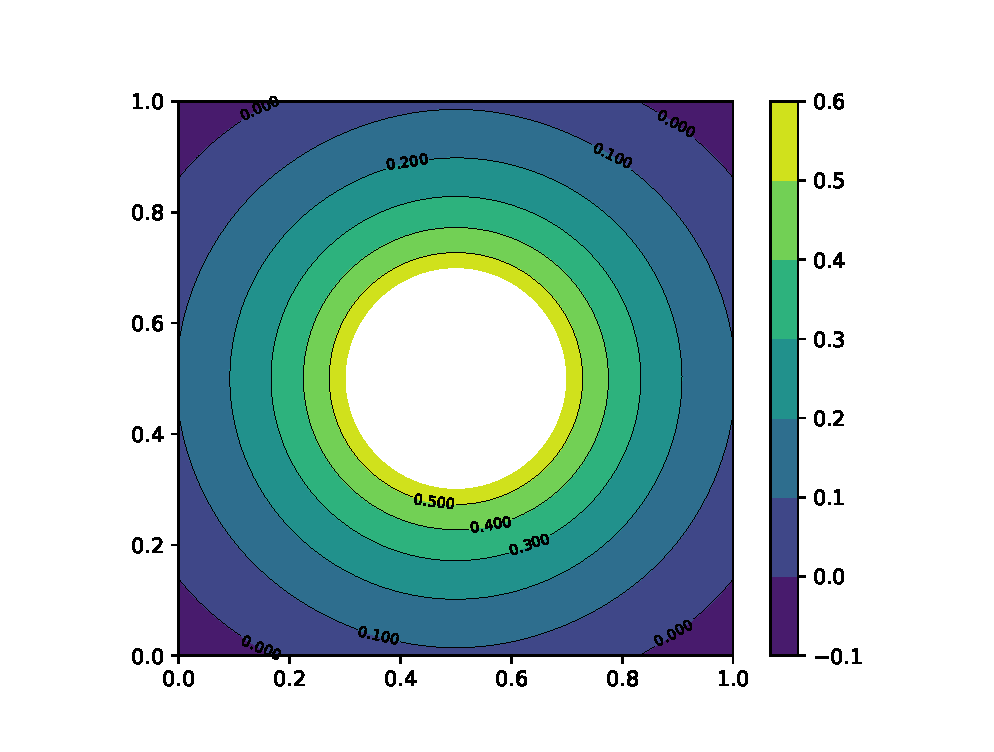
\includegraphics[width=1\linewidth]{phi_endf}
            \\ б) $\varphi$
        \end{minipage}
        \label{fig:4_4:6}
    \end{figure}
    Начальное значение функционала качества $0.045$
    после тридцати итераций становится равным $6.2\cdot10^{-5}$.
\end{frame}
\note{
    63. Квадрат с полостью внутри. (не доступная среда).
}
\begin{frame}
    \frametitle{Исследование устойчивости решений обратных задач с данными Коши}
    Положим $a\partial_n \theta = q_b +\varepsilon \psi$, где $\psi = \psi(x)$, $x \in \Gamma_1$ функция возмущения.

    Полученное решение задачи~\eqref{eq:2_4:eq2},~\eqref{eq:2_4:bc3} обозначим за $\theta^{\varepsilon}$.
    $\theta$ будет соответствовать случаю $\varepsilon = 0$.

    Область $\Omega$ -- квадрат с единичной стороной, $\Gamma_1$ соответствует стороне $y = 1$.

    Положим $\theta_b = (x + y) / 2$ и $q_b = a / 2$, $\varepsilon \in [-0.1, 0.1]$,
    вычислим $L^2$ норму отклонения возмущенного поля.
    \begin{figure}[h!t]
        \begin{minipage}[b][][b]{0.4\linewidth}
            \centering
            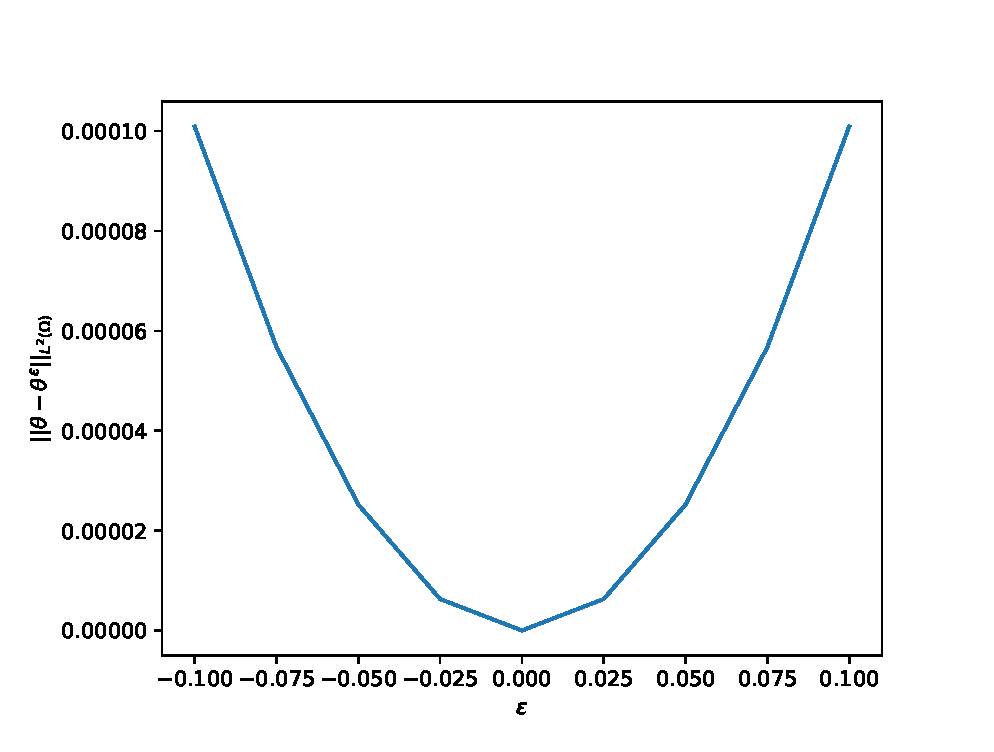
\includegraphics[width=1\linewidth]{additional/2/deps_1}\\ а) $\psi = 1,$
        \end{minipage}
        \hfill
        \begin{minipage}[b][][b]{0.4\linewidth}
            \centering
            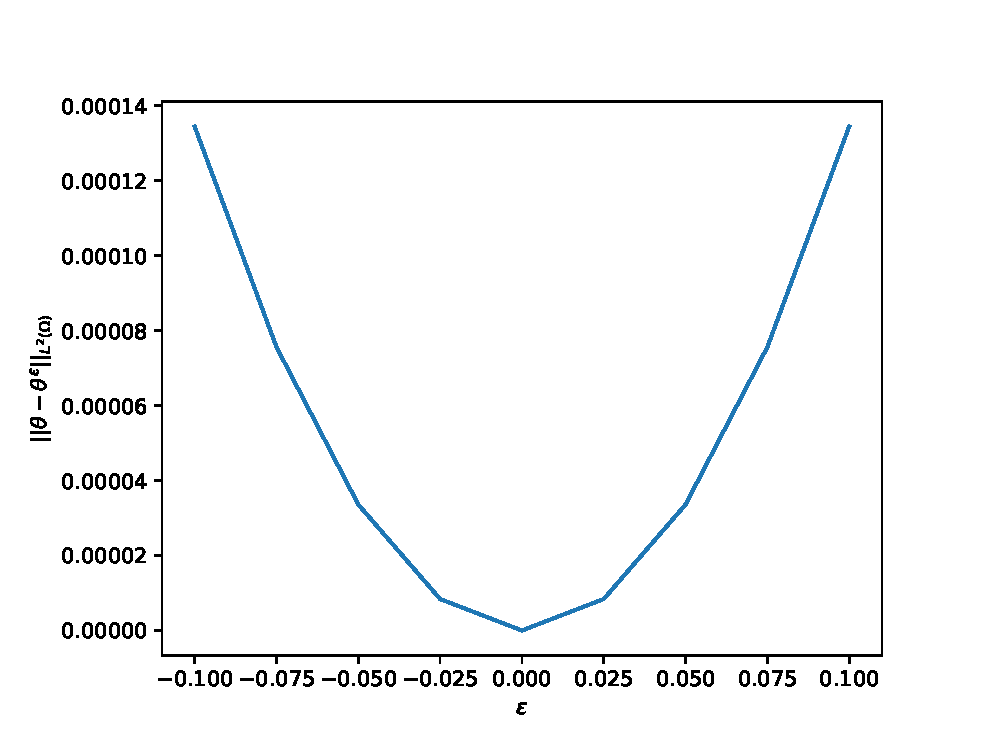
\includegraphics[width=1\linewidth]{additional/2/eps_sin} \\ б) $\psi = \sin (100 * \pi x)$.
        \end{minipage}
        \caption{$||\theta^\varepsilon - \theta||_{L^2(\Omega)}$}
        \label{fig:4_4:vareps}
    \end{figure}
    Численные эксперименты демонстрируют
    устойчивость решения относительно изменений теплового потока.
\end{frame}
\note{
    Также приведем результаты по исследованию устойчивости решений
    обратных задач с данными Коши.
    Для этого переопределим в уравнении~\eqref{eq:2_4:bc3} $a\partial_n \theta = q_b +\varepsilon \psi$,
    где $\psi = \psi(x), x \in \Gamma_1$ некоторая функция, моделирующая возмущение.
    Полученное таким образом решение задачи~\eqref{eq:2_4:eq2},~\eqref{eq:2_4:bc3}
    обозначим за $\theta^{\varepsilon}$.
    Следовательно, $\theta$ будет соответствовать случаю $\varepsilon = 0$.
    Для проведения численного моделирования область $\Omega$ определим
    как квадрат с единичной стороной, где $\Gamma_1$ соответствует стороне $y = 1$.
    Положим $\theta_b = (x + y) / 2$ и $q_b = a / 2$ соответственно.
    Выполним расчеты температурного поля
    для различных малых значений параметра возмущений $\varepsilon$
    из промежутка $[-0.1, 0.1]$ и вычислим $L^2$ норму отклонения возмущенного поля.


    Хорошо известно, что решение задачи с данными
    Коши на границе для одного эллиптического уравнения,
    напр.\ уравнения Лапласа, неустойчиво
    (знаменитый пример Адамара, когда малые изменения
    теплового потока на границе приводят к большим изменениям решения).
    Для рассматриваемой новой модели сложного теплообмена с данными Коши
    теоретический анализ устойчивости это открытая проблема.

    На первом этапе этот вопрос был исследован численно с использованием
    разработанного комплекса программ.

    Полученные численные результаты позволяют высказать гипотезу
    об устойчивости решения этой модели, которую в дальнейшем планируется обосновать аналитически.

}


\section{Задачи оптимального управления для квазилинейных моделей}\label{sec:opt}

\subsection{Задачи оптимального управления с ограничениями на состояние системы и метод штрафа}\label{subsec:opt-phase}
\begin{frame}
    \frametitle{Квазилинейная модель c фазовыми ограничениями}
    \begin{wrapfigure}{r}{0.34\textwidth}
        \centering{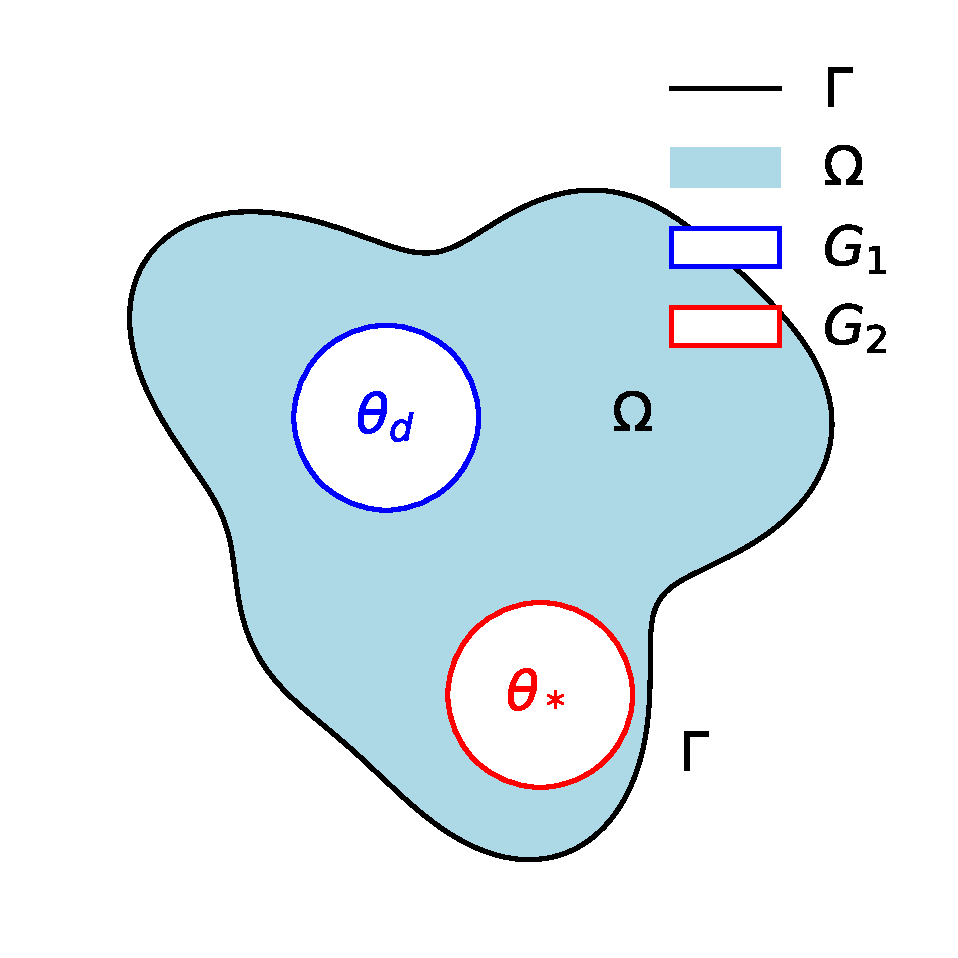
\includegraphics[width=1\linewidth]{omega-g1-g2}}
%        \caption*{$\Gamma \coloneqq \partial \Omega =\overline{\Gamma}_0 \cup \overline{\Gamma}_1 \cup \overline{\Gamma}_2$}
    \end{wrapfigure}

    \textbf{Задача оптимального управления $P$} заключается в минимизации функционала
    \[ J(\theta)=\int_{0}^{T} \int_{G_{1}}\left(\theta-\theta_{d}\right)^{2} dx dt \rightarrow \inf \]
    на решениях начально-краевой задачи:
    \begin{equation}
        \label{eq:3_2:1}
        \begin{gathered}
            \sigma \partial \theta / \partial t-\operatorname{div}(k(\theta)
            \nabla \theta)-\beta \varphi=u_{1} \chi \\
            -\operatorname{div}(\alpha \nabla \varphi)+\beta \varphi=u_{2}
            \chi, \quad x \in \Omega, \quad t \in(0, T),
        \end{gathered}
    \end{equation}
    \begin{equation}
        \label{eq:3_2:2}
        \theta=\left.0\right|_{\Gamma},
        \quad \alpha \partial_{n} \varphi
        +\left.2^{-1} \varphi\right|_{\Gamma}=0,
        \left.\quad \theta\right|_{t=0}=\theta_{0}.
    \end{equation}
    При этом учитываются ограничения:
    \[ u_{1,2} \geq 0, \quad u_{1}+u_{2} \leq P, \left.\quad \theta\right|_{G_{2}} \leq \theta_{*} \]

    \textbf{Задача со штрафом $P_{\varepsilon}$}.
    $J_{\varepsilon}(\theta) \rightarrow \inf$, где
    \[
        \begin{aligned}
            & J_{\varepsilon}(\theta)=\int_{0}^{T}
            \int_{G_{1}}\left(\theta-\theta_{d}\right)^{2} dx dt
            +\frac{1}{\varepsilon} \int_{0}^{T}
            \int_{G_{2}} F(\theta) d x d t, \\
            & \sigma \theta^{\prime}+A(\theta)=u,
            \quad \theta(0)=\theta_{0}, \quad u \in U_{a d},\\
            &F(\theta)=
            \begin{cases}
                0, & \text { если } \theta \leq \theta_{*} \\
                \left(\theta-\theta_{*}\right)^{2},
                & \text { если } \theta>\theta_{*}.
            \end{cases}
        \end{aligned}
    \]

\end{frame}
\note{
    Дана область, в ней две подобласти. Мы хотим в одной достичь определенного температурного режима,
    в другой хотим не допустить превышения заранее заданного ограничения.
    $P$ – максимальная мощность источника,
    $\alpha$ – коэффициент диффузии фотонов,
    $Hi$ есть характеристическая функция той части среды, в которой он расположен, деленная на его объём.
    $\beta$ – коэффициент поглощения, $k(\theta)$ является коэффициентом теплопроводности,
    $\sigma$ является произведением удельной теплоемкости и плотности среды,
    $u_1$ описывает мощность источника тепла, $u_2$ – мощность источника теплового излучения.

    Главная проблема здесь-наличие ограничения на температуру в области $G_2$.
    Для ее преодоления рассматривается задача со штрафом.
    Нарушение указанного ограничения штрафуется ростом функционала при малых значениях $\epsilon$.
    Обоснована сходимость предложенного штрафного алгоритма к решению задачи
    с ограничениями на температуру при $\epsilon\to+0$.
}
\begin{frame}
    \textbf{Условия разрешимости и сходимость решений при $\varepsilon \rightarrow +0$}
    \begin{itemize}
        \item $(c1)\; \sigma_{0} \leq \sigma \leq \sigma_{1}, \quad|\partial \sigma / \partial t| \leq \sigma_{2}$
        \item $(c2)\; k_{0} \leq k(s) \leq k_{1}, \quad\left|k^{\prime}(s)\right| \leq k_{2}, \quad s \in \mathbb{R}$,
        \item $(c3)\; \theta_{0} \in L^2(\Omega)$
        \item $(c4)\; \alpha_{0} \leq \alpha(x) \leq \alpha_{1}, \beta_{0} \leq \beta(x) \leq \beta_{1}, \quad x \in \Omega$,
    \end{itemize}
    \begin{theorem}[3.1]
        \label{th:3_2:1}
        Пусть выполняются условия $(c1)$-$(c3)$, и $\theta_{0} \leq \theta_{*}$ п.\ в. в $\Omega$.
        Тогда существует решение задачи $P$.
    \end{theorem}
    \begin{theorem}[3.2]
        \label{th:3_2:2}
        Пусть выполняются условия $(c1)$-$(c4)$.
        Тогда существует решение задачи $P_{\varepsilon}$.
    \end{theorem}
    \begin{theorem}[3.3]
        \label{th:3_2:3}
        Пусть выполнены условия $(c1)$-$(c4)$, и $\theta_{0} \leq \theta_{*}$ п.\ в. в $\Omega$.
        $\left\{\theta_{\varepsilon}, u_{\varepsilon}\right\}$ -- решение задачи
        $P_{\varepsilon}$ для $\varepsilon>0$, тогда существует последовательность $\varepsilon \rightarrow+0$
        \[
            u_{\varepsilon} \rightarrow \widehat{u} \text { слабо в } L^{2}(0, T ; H), \quad
            \theta_{\varepsilon} \rightarrow \widehat{\theta} \text { сильно в } L^{2}(0, T ; H),
        \]
        где $\{\widehat{\theta}, \widehat{u}\}$ есть решение задачи $P$\@.
    \end{theorem}
\end{frame}
\begin{frame}
    \textbf{Моделирование влияния коэффициента $k(\theta)$ на динамику температурного поля}
    В первом эксперименте для~\eqref{eq:3_2:1}--\eqref{eq:3_2:2} параметр $k$ определим как
    $ k(\theta)=
    \begin{cases}
        0.1, & \text { если } \theta \leq \theta_{*}, \\
        1, & \text { если } \theta>\theta_{*},
    \end{cases}
    $
    а также определим $\theta_b = 1$ на всей границе.
    Во втором эксперименте положим $\theta_b = (x + y) /2$ и
    $k(\theta)=
    \begin{cases}
        0.1, & \text { если } \theta \leq 0.5, \\
        m_1, & \text { если } \theta > 0.5.
    \end{cases}
    $
    \begin{figure}[h!t]
        \begin{minipage}[b][][b]{0.49\linewidth}
            \centering
            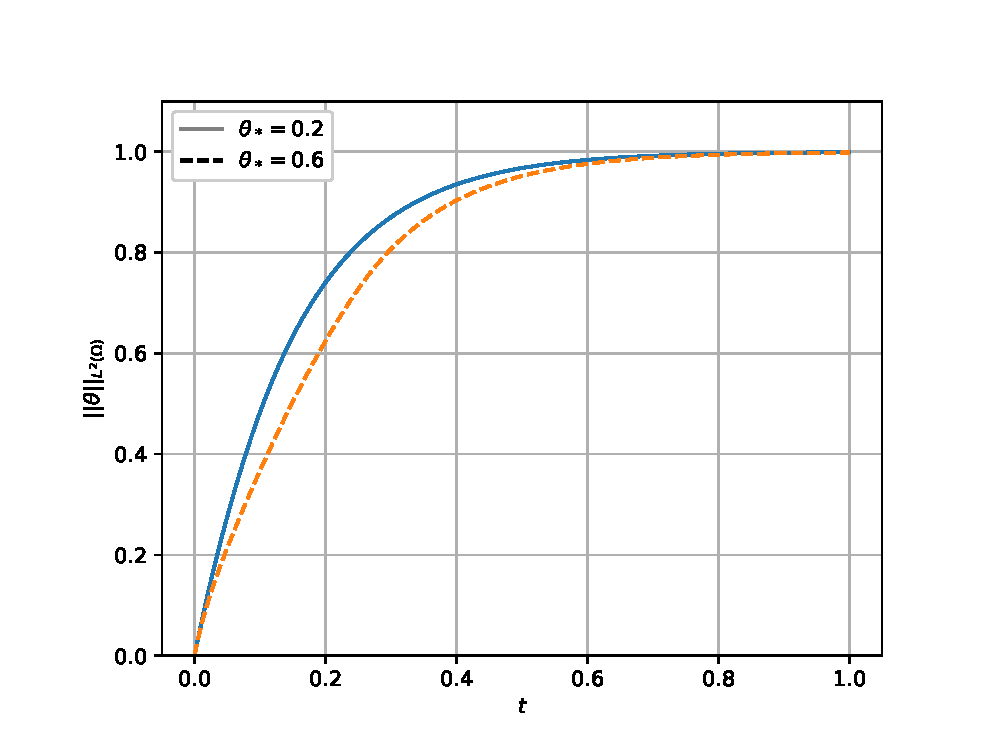
\includegraphics[width=1\linewidth]{additional/3/theta_dyn_star} \\ а) Первый эксперимент
        \end{minipage}
        \hfill
        \begin{minipage}[b][][b]{0.49\linewidth}
            \centering
            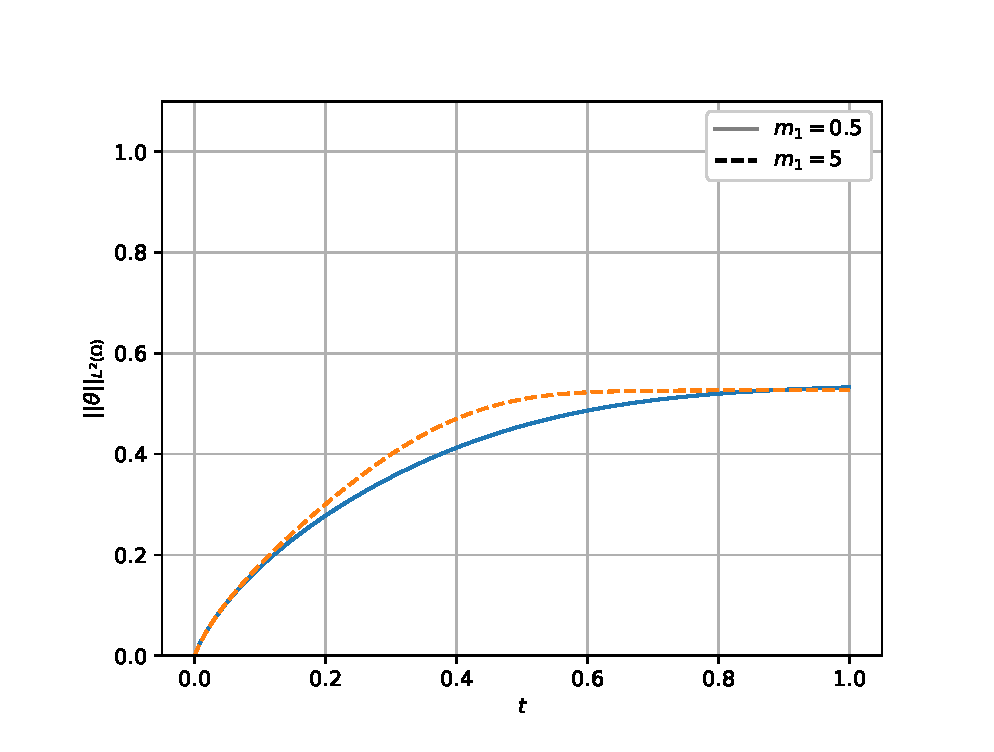
\includegraphics[width=1\linewidth]{additional/3/theta_dyn_m} \\ б) Второй эксперимент
        \end{minipage}\label{fig:figure~~}
    \end{figure}
\end{frame}
\note{
    В рассмотренной модели коэффициент теплопроводности зависит от
    неизвестной температуры (квазилинейность уравнения).
    Это позволяет моделировать эффекты переноса энергии в областях с высокой температурой.
    Разработанный комплекс программ позволяет оценить
    влияние этого коэффициента на динамику темп поля.
    температурного поля

    Здесь показать анимацию.
}
       % Настройки заглавной странице
\begin{frame}
    \frametitle{Научная новизна}
    \begin{itemize}
        \item Получены новые априорные оценки решений начально-краевых задач для
        квазистационарных и квазилинейных уравнений сложного теплообмена и до
        казана их нелокальная однозначная разрешимость.
        \item Представлены априорные
        оценки решений регуляризованных задач и обоснована сходимость их решений к
        точным решениям обратных задач.
        \item Для решения задач с фазовыми ограничениями,
        предложены алгоритмы, основанные на аппроксимации экстремальными
        задачами со штрафом.
        \item Реализованы программные комплексы
        \begin{enumerate}
            \item По решению обратных задач, основанные на оптимизационных методах
            \item Тестирования решений, получаемых в результате решения обратных задач
            \item Инструменты моделирования процессов сложного теплообмена для манипуляции `in place`
            \item Инструменты визуализации получаемых значений в процессе моделирования
        \end{enumerate}
    \end{itemize}
    \begin{minipage}[t]{.25\linewidth}
        \center{
\includegraphics[width=1\linewidth]{reg1}}
    \end{minipage}
    \hfill
    \begin{minipage}[t]{.25\linewidth}
        \center{
\includegraphics[width=1\linewidth]{reg2}}
    \end{minipage}
    \hfill
    \begin{minipage}[t]{.25\linewidth}
        \center{
\includegraphics[width=1\linewidth]{reg3}}
    \end{minipage}
\end{frame}
\note{
    В работе получены новые априорные оценки решений
    начально-краевых задач для квазистационарных и квазилинейных
    уравнений сложного теплообмена и доказана их нелокальная однозначная
    разрешимость.
    Для рассмотренных моделей сложного теплообмена
    рассмотрены новые постановки граничных обратных задач, предложены
    оптимизационные методы их решения.
    Выполнен теоретический анализ возникающих новых экстремальных задач.
    Представлены априорные оценки решений регуляризованных задач и впервые
    обоснована сходимость их решений к точным решениям обратных задач.
    Для решения задач с фазовыми ограничениями, предложены алгоритмы,
    основанные на аппроксимации экстремальными задачами со штрафом.
    Разработаны и протестированы новые алгоритмы решения прямых,
    обратных и экстремальных задач для моделей сложного теплообмена.
}



\begin{frame} % публикации на одной странице
    \frametitle{Публикации, конференции}
    ВАК:
    \small{
        \begin{enumerate}
            \item P. R. Mesenev\ — \textit{Дальневост. матем. журн.} 23.1 (2023).

            \item П. Р. Месенев и А. Ю. Чеботарев
            — \textit{Ж. вычисл. матем. и матем. физ.} (2023).

            \item P R Mesenev and A Yu Chebotarev
            — \textit{Comput. Math. Math. Phys. 62.1} (Jan. 2022).

            \item A. Yu. Chebotarev, N. M. Park, P. R. Mesenev и A. E. Kovtanyuk
            — \textit{Dal’nevostochnyi Matematicheskii Zhurnal} (2022).

            \item A. Yu. Chebotarev и P. R. Mesenev
            — \textit{Dal’nevostochnyi Matematicheskii Zhurnal} (2020).

            \item P. R. Mesenev и A. Yu. Chebotarev
            — \textit{Dal’nevostochnyi Matematicheskii Zhurnal} (2018).
        \end{enumerate}
    }
    Прочее:
    \small{
        \begin{enumerate}
            \item A. Chebotarev, A. Kovtanyuk, P. Mesenev
            — \textit{Proceedings
            of the Workshop on Mathematical Modeling and Scientific Computing:
            Focus on Complex Processes and Systems – Dedicated to the Memory of
            Nikolai Botkin} (2020).

            \item A Yu Chebotarev, N M Park, P R Mesenev и A E Kovtanyuk
            — \textit{ Journal of Physics: Conference Series} (2023).

            \item A. Chebotarev, P. Mesenev и A. Kovtanyuk
            — \textit{2023 Days on Diffraction (DD)} (2023).

            \item A. Chebotarev, A. Kovtanyuk, N. Park, P. Mesenev
            — \textit {2021 Days on Diffraction (DD)} (2021).

            \item П. Р. Месенев
            — \textit{Материалы региональной научно-практической
            \item конференции студентов, аспирантов и молодых учёных по
            естественным наукам} (2018)
        \end{enumerate}
    }

    Конференции:
    \small{
        \begin{itemize}
            \item Региональная научно-практическая конференция (Владивосток, 2018, 2019);
            \item Workshop on Computing Technologies and Applied Mathematics (Владивосток, 2022);
            \item Int.\ Conference DAYS on DIFFRACTION (Санкт-Петербург, 2021, 2023);
            \item Int.\ Workshop on Math.\ Modeling and Scientific Computing (Мюнхен, 2020, 2022).
        \end{itemize}
    }
\end{frame}
    % Последние слайды презентации
\appendix
%\begin{frame}
%    \frametitle{Ответы на замечания ведущей организации НИИ~<<Рога~и~копыта>>}
%    \begin{itemize}
%        \item Замечание -- ответ
%        \item Замечание -- ответ
%        \item Замечание -- ответ
%        \item Замечание -- ответ
%        \item Замечание -- ответ
%    \end{itemize}
%\end{frame}
%
%\begin{frame}
%    \frametitle{Ответы на замечания оф. оппонента Иванова\,И.\,И}
%    \begin{itemize}
%        \item Замечание -- ответ
%        \item Замечание -- ответ
%        \item Замечание -- ответ
%        \item Замечание -- ответ
%        \item Замечание -- ответ
%    \end{itemize}
%\end{frame}
%
%\begin{frame}
%    \frametitle{Ответы на замечания Петрова\,П.\,П}
%    \begin{itemize}
%        \item Замечание -- ответ
%        \item Замечание -- ответ
%        \item Замечание -- ответ
%        \item Замечание -- ответ
%        \item Замечание -- ответ
%    \end{itemize}
%\end{frame}
      % Запасные слайды презентации
\end{document}
